\documentclass[a4paper, twoside]{article}
\usepackage[fontsize=11pt]{scrextend}
%\documentclass[10pt]{extarticle}
\usepackage[T1]{fontenc}
\usepackage[utf8]{inputenc}

\usepackage[margin=1in]{geometry}
\usepackage{amsfonts, amsmath, amssymb}
\usepackage{mathtools}

\usepackage{pifont}


\usepackage{graphicx}
\usepackage{subfig}
\usepackage{epsfig}
\usepackage{color}

\graphicspath{{/hdd/Documents/math-cnn-derivation-swedish-paper/English/images}}

\usepackage{url}
%%  Defines the command \url{} that can be used to typeset url:s
%%  in text

\usepackage[parfill]{parskip}
\usepackage{ragged2e}

\setcounter{tocdepth}{4}
\setcounter{secnumdepth}{4}


\newcommand*{\pd}[2]{\ensuremath{\dfrac{\partial #1}{\partial #2}}}
\newcommand*{\inpd}[2]{\ensuremath{\frac{\partial #1}{\partial #2}}}
\DeclarePairedDelimiter\floor{\lfloor}{\rfloor}

\title{Dense face detection and improving temporal convolutional networks for automatic image captioning}
\author{Nikita Zozoulenko \\*
nikita.zozoulenko@gmail.com \\*
Katedralskolan Linköping\\*
Supervisor: Oleg Burdakov \\*}

\begin{document}
\maketitle

\vfill
\begin{figure}[h]
    \centering
    \subfloat[Dense Face Detection]{{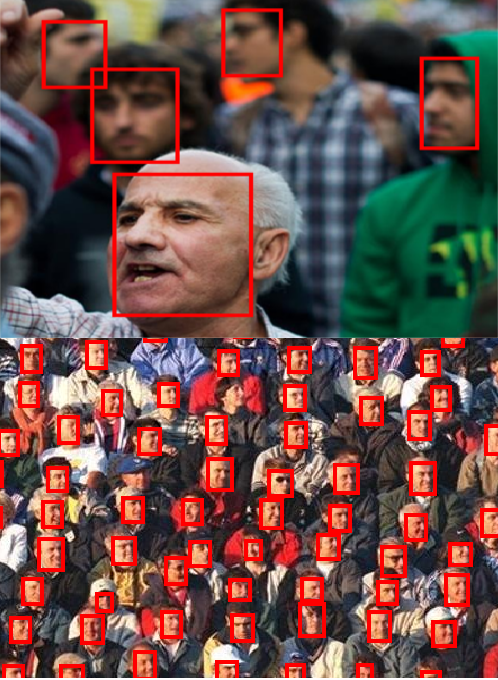
\includegraphics[width=7.5cm]{frontface.png} }}
    \subfloat[Automatic Image Captioning]{{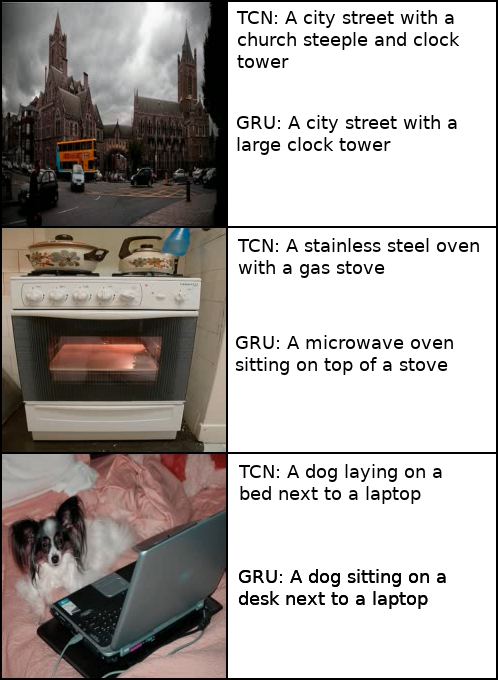
\includegraphics[width=7.605cm]{captionssmall.png} }}
  	\caption{(a) The proposed convolutional-neural-network-based model FaceNet is capable of dynamically detecting up to hundreds of faces in a crowded scene for various scales, lighting and occlusions. (b) A temporal convolutional neural network (TCN) and a Gated Recurrent Unit (GRU) automatically captioning an image.} \label{figtitle}
\end{figure}
\vfill

\newpage

%start abstract
\Large{\textbf{Abstract}}\\
\normalsize{}
Convolutional neural networks (CNNs) are traditionally used in computer vision, but have recently gained traction as sequential models. I suggested two improvements to temporal convolutional networks (TCNs) and empirically evaluated them to achieve a new state of the art on the task of SequenceMNIST (99.53\% versus 99.0\%) and Permuted SequenceMNIST (97.86\% versus 97.28\%). Three different residual blocks were also experimented on to find the effect of residual connections on the performance of TCNs. The improved model was then compared to its recurrent neural network counterpart, a Gated Recurrent Unit, on an area where TCNs have never been applied before; automatic image captioning, and is shown to perform similarly. Additionally, since the field lacks a fully derived order 4 example of a CNN, I presented a clear derivation of the general case for a CNN with an arbitrary input of a tensor of order 4, including varying zero-padding and strides during forward and backpropagation. The derivation was then used for my own neural network library implementation in Python and C++. Furthermore, I systematically construct a region based dense face detector and empirically investigate how factors such as cross entropy loss, focal loss, feature pyramid networks, online hard example mining, color jitter, and network depth affects its performance. The final model is sufficiently accurate and computationally efficient to be used for real time video, for instance CCTV or other surveillance systems.

\newpage
%end abstract

\tableofcontents
\newpage
\section{Introduction}

An Artificial neural network is a biologically inspired machine learning model that draws inspiration from the biologial brain in mammals. Artificial neural networks can vary in structure and architecture, but the basic principle behind neural networks is that they are made up of a number of layers of neurons. The layers are built sequentially such that the output of one layer is the input to the next layer. The number of layers a neural network is constructed out of is called its depth. How the neurons of the previous layer are connected to the neurons of the next layer depends on the specific type of artificial neural network \cite{cs231n}.

Similar to other machine learning models, an artificial neural network wants to predict a predetermined number of values, given a number of input features. For instance, a neural network can be given all the pixel values in an image and classify the content in the image. The neural network is trained to predict accurate predictions through supervised learning. Data pre-labeled by humans is used to supervise the training. The model is given input data and is asked to predict values as close to the human label as possible. The model does this by optimizing a number of learnable parameters at every layer in the neural network. The human label is called the ground truth of the data \cite{cs231n}.

Artificial neural networks, or more specifically convolutional neural networks, were popularized 2012 when the model was used to win the annual ImageNet Large-Scale Visual Recognition Challenge, beating all current machine learning models. Today convolutional neural networks have achieved the state of the art in areas such as self-driving cars, image classification, object localization, automatic image annotation, semantic segmentation of objects in images and natural language processing \cite{cs231n}.

\subsection{Background}
\subsection{Feed-forward neural networks}
A feed-forward neural network is the most elementary version of an artificial neural network. As all varying kinds of artificial neural networks, a feed-forward neural network is made out of a number of layers of neurons. The unique property of a feed-forward neural network is that all the neurons in a layer are connected to every neuron in the next layer (see figure \ref{figfeedforward}) \cite{cs231n}.

\begin{figure}[h]
	\centering
  		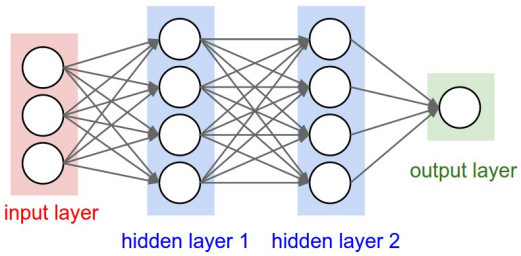
\includegraphics[scale=1]{feedforward.png}
  	\caption{An illustration \cite{hidden12} of a simple feed-forward neural network. It consists of four layers: an input layer (red), two hidden layers (blue) and one output layer (green). A circle represents a neuron. Every neuron in a layer is connected to all the neurons in the following layer, shown by the grey lines between the neurons. } \label{figfeedforward}
\end{figure}

A neuron is represented by a floating point decimal number. The value of a neuron is called its activation. Given an input of $n$ features, the model wants to predict $m$ different values. $n$ and $m$ are set as the size and number of neurons in the input and output layer respectively. The values of the input neurons are transferred to the next layer depending on the strength of the connection between every pair of neurons in two adjacent layers. This is done for every layer until the signal has reached the output layer. The process of propagating the values of the input neurons to the output layer is called forward propagation \cite{cs231n}.

The network is trained to predict correct values by optimizing the fixed connections, also called weights, between every pair of neurons in two consecutive layers in the neural network \cite{cs231n}.

\subsubsection{Tensors, indexing and notation}
A tensor is the generalization of vectors and matrices. Scalars are tensors of order 0. A tensor of order 1 is a row vector $x \in \mathbb{R}^N$ with $N$ elements. It can also be seen as a one-dimensional array. Matrices $M$ are tensors of order 2 such that $M \in \mathbb{R}^{R \times N}$ and can be viewed as vectors with $R$ elements where every element is another vector with $N$ scalar elements. Matrices can also be seen as a two-dimensional array with $RN$ elements. A tensor of order $n$ is an $n$-dimensional array and is indexed by an $n$-tuple. For instance, a tensor $X \in \mathbb{R}^{R \times C \times H \times W}$ is indexed by the four-tuple $(r,c,h,w)$ where $1 \leq r \leq R$, $1 \leq c \leq C$, $1 \leq h \leq H$ and $1 \leq w \leq W$ \cite{cs231n}.

\subsubsection{Forward propagation}
Input data is forward propagated in in mini-batches of $R$ examples at a time. Let $L$ denote the number of layers in the neural network and $l$, $1 \leq l \leq L$, one specific layer in the neural network. $N^{(l)}$ is the number of neurons in layer $l$. The values of the neurons of layer $l$, called the layer's activations, are expressed as a tensor of order 2: $X^{(l)} \in \mathbb{R}^{R \times N^{(l)}}$ indexed by the two-tuple $(r,i)$ where $1 \leq r \leq R$ and $1 \leq i \leq N^{(l)}$. In addition to the neurons of layer $l$, there is a bias neuron $b^{(l)} \in \mathbb{R}$ (see figure \ref{figFCCmath}). It is called a bias neuron because its value is independent to what input the neural network is given \cite{cs231n} \cite{wikiStanford}.

The weights representing the strength of the connections between the neurons of layer $l$ and $l+1$ are also expressed as a tensor of order 2. Let $W^{(l)} \in \mathbb{R}^{N^{(l+1)}  \times N^{(l)}}$ such that the element $W_{j, i}^{(l)}$ is the strength of the connection between neuron $X_{ri}^{(l)}$ and $X_{rj}^{(l+1)}$ for arbitrary example $r$ in the mini-batch \cite{cs231n} \cite{wikiStanford}.

\begin{figure}[h]
	\centering
  		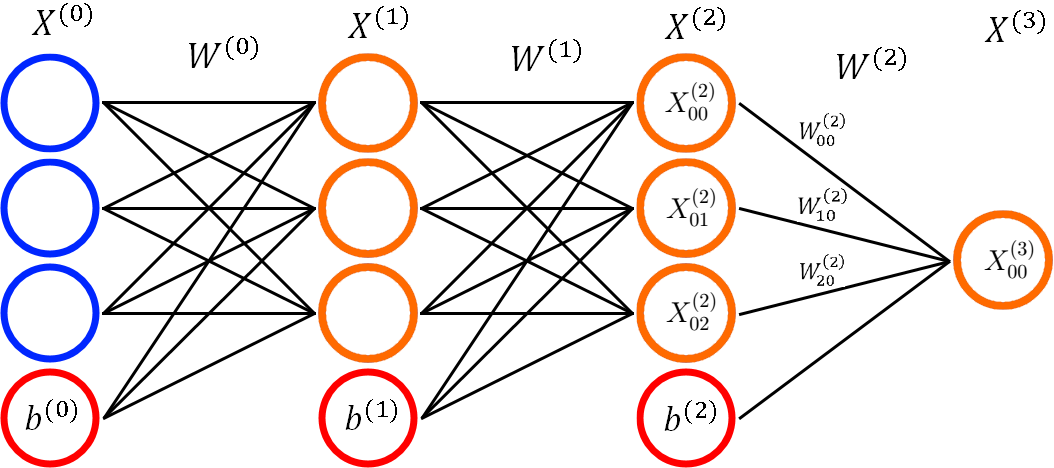
\includegraphics[scale=0.4]{FCC.png}
  	\caption{An example of a 4 layer feed-forward neural network. The input neurons are marked with blue. The bias neurons are marked with red. Black lines between neurons symbolyze the weights between every pair of neurons between two layers.} \label{figFCCmath}
\end{figure}

The calculation of the value of a neuron in layer $l+1$ includes computing the sum of every neuron in layer $l$ multiplied with its corresponding weight in $W^{(l)}$, plus the value of the bias $b^{(l)}$. The sum is then put in a so called activation function $f$. The value of the activation function is the neuron's activation in layer $l+1$ \cite{cs231n} \cite{wikiStanford}.

Let $Z^{(l)} \in \mathbb{R}^{R \times N^{(l)}}$ be the value of each neuron in layer $l$ before being put into the activation function. Given an input $X^{(1)}$ the forward propagation is expressed recursively as \cite{cs231n} \cite{wikiStanford}:

\begin{align}
Z_{rj}^{(l+1)} & = b^{(l)} + \sum^{N^{(l)}}_{i = 1} X^{(l)}_{r,i} W^{(l)}_{i,j}\\
X_{rj}^{(l+1)} & = f(Z_{rj}^{(l+1)})
\end{align}

The tensor of activations and weights are constructed in such a way that one forward pass through a single layer can be computed with a single dot product and an addition of the bias term added to every element. The activation function $f$ is then applied element-wise on each neuron \cite{cs231n} \cite{wikiStanford}:

\begin{align}
Z_{rj}^{(l+1)} & = \begin{bmatrix}
X^{(l)}W^{(l)}
\end{bmatrix}_{rj}+b^{(l)} \\
X_{rj}^{(l+1)} & = f(Z_{rj}^{(l+1)})
\end{align}

Common activation functions are Rectified Linear Units (ReLU), sigmoid ($\sigma$) and hyperbolic tangent ($\tanh$) and are defined by equations \eqref{relu} - \eqref{tanh} (see figure \ref{activation_function}). A non-linear activation function is chosen to enable the network to make use of non-linearities when learning to predict values. Without non-linear activation functions, the whole model is equivalent to one large linear transformation of the input data \cite{cs231n}.
\\
\begin{figure}[h]
	\centering
  		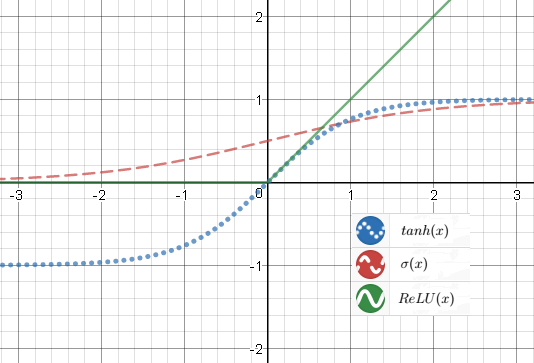
\includegraphics[scale=0.73]{activationfunction.png}
  	\caption{A graph of ReLU, $\sigma$ and $\tanh$.} \label{activation_function}
\end{figure}

\begin{equation}\label{relu}
\mbox{ReLU}{(x)} = \begin{cases} 
			0 & \mbox{if } x < 0 \\ 
			x & \mbox{if } x \geq 0 
		\end{cases}
\end{equation}

\begin{equation}\label{sigmoid}
\sigma(x) = \frac{1}{1+e^{-x}}
\end{equation}

\begin{equation}\label{tanh}
\tanh{(x)} = \frac{e^x-e^{-x}}{e^x+e^{-x}}
\end{equation}

\subsubsection{Loss function}
Given an input $X \in \mathbb{R}^{R \times N^{(1)}}$ and a ground truth $y \in \mathbb{R}^{R \times N^{(L)}}$ the model wants to predict values $\hat{y}$ which resembles the ground truth as closely as possible. It is achieved by defining a multivariate loss function $L(\theta; X, y)$  with the network's parameters $\theta$ (all the weights and biases) with respect to a single training mini-batch $(X, y)$. The loss function describes the quality of the neural network's prediction $\hat{y}$ such that a lower loss represents a more accurate prediction. $\hat{y}$ is synonymous with the activations of the last layer $L$ in the network and is a function of the parameters $\theta$ of the network and the input data $X$. $y$ is the human labeled ground truth with the same dimensionality as $\hat{y}$. To simplify noration $L(\theta)$ is used to denote the loss function with respect to one mini-batch $(X, y)$ of training data. One way of defining the loss function is to use the mean squared error defined by the following equation \cite{cs231n}:

\begin{equation}\label{MSE}
L(\theta) = \frac{1}{RN^{(L)}} \sum^{R}_{r=1} \sum^{N^{(L)}}_{i=1} (\hat{y}_{r,i}-y_{r,i})^2
\end{equation}

Here $R$ is the batch size and $N^{(L)}$ is the number of neurons in the last layer $L$.

The process of minimizing the loss function is called training. The model iterates through supervised training data and calculates the loss with respect to a mini-batch of training examples. Since the given input $X$ and ground truth $y$ stays fixed, the network learns by optimizing its weights $W^{(l)}$ and biases $b^{(l)}$ for every layer $l$ to decrease the loss \cite{cs231n} \cite{wikiStanford}.

\subsubsection{Gradient Descent}
The gradient $\nabla L(\theta)$ is a vector of partial derivatives with respect to the parameters $\theta$ of the function $L$ defined by the following equations \cite{gradient} \cite{convmath}:
\begin{equation}\label{EQgradientspace}
\nabla L(\theta) : \mathbb{R}^n \to \mathbb{R}^n
\end{equation}
\begin{equation}\label{EQgradientvector}
\nabla L(\theta) = 
	\begin{pmatrix} 
		\pd{L(\theta)}{\theta_{1}}, & 
		\pd{L(\theta)}{\theta_{2}}, &
		\cdots, &
		\pd{L(\theta)}{\theta_{n}}
		
		\end{pmatrix}
\end{equation}

The gradient $\nabla L(\theta)$ shows the direction of steepest ascent in the point ($\theta_{1}$, $\theta_{2}$, ..., $\theta_{n}$) in the $n$-dimensional vector space $\mathbb{R}^{n}$. For a function $f(x)$ of a single variable $x$, the gradient is simply the derivative of the function with respect to $x$ and is the slope of the tangent line to $f$ at $x$. For a function $f(x,y)$ of two variables $x$ and $y$, the gradient is the two-dimensional vector of the slope in the $x$ dimension and $y$ dimension respectively. The loss function used in neural networks can be a function of millions of parameters, depending on the depth and size of the neural network \cite{gradient} \cite{convmath}.

Gradient descent is the method of iteratively changing the values of the parameters $\theta$ proportionally to the negative gradient $-\nabla L(\theta)$ to minimize the function $L(\theta)$ (see figure \ref{figSGD}). The most basic algorithm of gradient descent is called Stochastic Gradient Descent (SGD) and uses the hyperparameter $\alpha$, called learning rate, to control the magnitude of the gradient. It is called Stochastic Gradient Descent because, at each iteration, the mini-batch responsible for the losses is randomly chosen and sampled from the whole batch of training data. Stochastic Gradient Descent is defined by the following equations \cite{wikiStanford} \cite{gradient} \cite{convmath}:

\begin{equation}\label{EQgradient}
\pd{L(\theta)}{\theta_i} = \nabla_{\theta_i} L(\theta)
\end{equation}
\begin{equation}\label{SGD}
{\theta_i} \to {\theta_i} - \alpha \pd{L(\theta)}{\theta_i}
\end{equation}

\begin{figure}[h]
	\centering
  		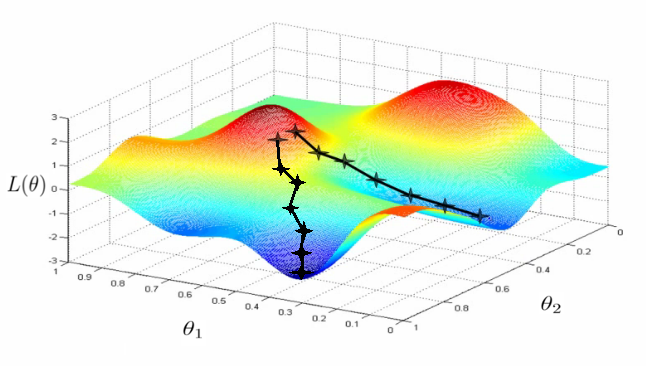
\includegraphics[scale=1]{gradient-descent.png}
  	\caption{An illustration \cite{figSGD} of Stochastic Gradient Descent on a function of two variables. Red regions symbolizes a high function value while blue regions symbolizes a low function value. The parameters were initialized near the global maximum and their values are altered iteratively to move in the direction of the negative gradient: the direction of steepest descent, to find a local minimum.} \label{figSGD}
\end{figure}

\subsubsection{Backpropagation}
Backpropagation is the process of calculating the partial derivatives of the loss function with respect to the model's parameters, or in other terms, the process of computing the gradient. The gradient is then used to modify the network's parameters to minimize the loss function \cite{wikiStanford} \cite{gradient}.

The partial derivatives can be approximated numerically with the formal definition of a derivative defined by the following equation \cite{wikiStanford} \cite{gradient}:

\begin{equation}\label{EQderivativeDefinition}
\pd{L(\theta)}{\theta_{i}} = \lim_{h \to 0} \frac{L(\theta_{1},...,\theta_{i} + h, ..., \theta_{n})-L(\theta)}{h}
\end{equation}

This would not be a problem for the small neural network in figure \ref{figFCCmath} with a total of 24 parameters, but would be extremely inefficient for deep neural networks with millions of parameters. Instead, the chain rule is applied to calculate the exact values of the partial derivatives in a computationally efficient manner \cite{cs231n}.

Let $\delta^{(l)}$ denote the so called delta-error at layer $l$, defined by the following equation:

\begin{equation}\label{deltaerrordefinition}
\delta^{(l)} = \inpd{L(\theta)}{X^{(l)}}
\end{equation}

The delta-error is the partial derivative of the loss with respect to a specific neuron in the model and is needed to efficiently compute the gradient with the help of the chain rule. The delta-error can be interpreted as how much a deviation in the value of a neuron affects the loss function. A change in value of a neuron with a big delta-error results in a greater change of the total loss compared to a neuron with a small delta-error. Because the activation of layer $l+1$ is a function of the previous layer $l$, the delta-error can be computed recursively from the output layer and propagated backwards to the first layer in the network. By applying the chain rule the delta-error $\inpd{L(\theta)}{X^{(l)}}$  at layer $l$ can be broken up into three partial derivatives $\inpd{L(\theta)}{X^{(l+1)}}$, $\inpd{X^{(l+1)}}{Z^{(l+1)}}$ and $\inpd{Z^{(l+1)}}{X^{(l)}}$. Since a single neuron in layer $l$ is connected to every neuron in layer $l+1$ you have to sum over every activation in layer $l+1$. The first partial derivative is the delta-error of the next layer and the other two partial derivatives are derived from equations (1) and (2) and are easily differentiable since (1) is a linear equation \cite{cs231n} \cite{wikiStanford}:
\begin{equation}\label{dLdX_FCC}
\begin{split}
\delta^{(l)}_{r,i}
	& = \pd{L(\theta)}{X^{(l)}_{r,i}}  \\
	& = \sum^{N^{(l+1)}}_{j=1} \pd{L(\theta)}{X^{(l+1)}_{r,j}} \pd{X^{(l+1)}_{r,j}}{Z^{(l+1)}_{r,j}} \pd{Z^{(l+1)}_{r,j}}{X^{(l)}_{r,i}} \\
	& = \sum^{N^{(l+1)}}_{j=1} \delta^{(l+1)}_{r,j} f'(Z^{(l+1)}_{r,i}) \ W^{(l)}_{j,i} 
\end{split}
\end{equation}

The delta-error of the last layer $L$ depends on the type of loss function used. For the mean squared error the delta-error of the output layer is defined by the following equation \cite{cs231n} \cite{wikiStanford}:

\begin{equation}\label{MSEdelta}
\begin{split}
\delta^{(L)}
	& = \pd{L(\theta)}{\hat{y}}  \\
	& = \frac{2}{RN^{(L)}} (\hat{y}-y)
\end{split}
\end{equation}

With the delta-error defined at every layer in the network the partial derivative of the loss function with respect to the networks parameters can be calculated. Just like equation (\ref{dLdX_FCC}), the chain rule is applied to break up $\inpd{L(\theta)}{X^{(l)}}$ into three partial derivatives, $\inpd{L(\theta)}{X^{(l+1)}}Potentially hazardous biological agents research:
a. Give source of the organism and describe BSL assessment process and BSL determination.
b. Detail safety precautions and discuss methods$, $\inpd{X^{(l+1)}}{Z^{(l+1)}}$ and $\inpd{Z^{(l+1)}}{W^{(l)}}$. All the examples in the mini-batch are summed over since the weights affect every single example. $\inpd{L(\theta)}{X^{(l+1)}}$ is the delta-error and the other two partial derivatives are derived from equations (1) and (2) \cite{cs231n} \cite{wikiStanford}:

\begin{equation}\label{dLdW_FCC}
\begin{split}
\pd{L(\theta)}{W^{(l)}_{j,i}} 
	& = \sum^{R}_{r=1} \pd{L(\theta)}{X^{(l+1)}_{r,i}} \pd{X^{(l+1)}_{r,i}}{Z^{(l+1)}_{r,i}} \pd{Z^{(l+1)}_{r,i}}{W^{(l)}_{i,j}} \\
	& = \sum^{R}_{r=1} \delta^{(l+1)}_{r,i} f'(Z^{(l+1)}_{r,i}) \ X^{(l)}_{r,j}\\
\end{split}
\end{equation}

The partial derivative of the loss function with respect to the biases are found in a similar way to equations (\ref{dLdX_FCC}) and (\ref{dLdW_FCC}) \cite{cs231n} \cite{wikiStanford}:
\begin{equation}\label{dLdb_FCC}
\begin{split}
\pd{L(\theta)}{b^{(l)}} 
	& = \sum^{R}_{r=1} \pd{L(\theta)}{X^{(l+1)}_{r,i}} \pd{X^{(l+1)}_{r,i}}{Z^{(l+1)}_{r,i}} \pd{Z^{(l+1)}_{r,i}}{b^{(l)}_{i,j}} \\
	& = \sum^{R}_{r=1} \delta^{(l+1)}_{r,i} f'(Z^{(l+1)}_{r,i}) \\
\end{split}
\end{equation}

\subsubsection{Training neural networks}
The model is trained by dividing the training data into mini-batches of size $R$. A mini-batch is then forward propagated and the loss is calculated. The loss is then used to backpropagate the model's deviation from the ground truth (the network's loss) layer by layer. Backpropagation starts at the output layer and propagates through the network backwards until it reaches the input layer. For every layer in the network the delta-error from the proceeding layer is used to calculate the new delta-error. It is then used to calculate the layers contribution to the total gradient by computing the partial derivatives with respect to the loss function. When the gradient has been fully computed, one iteration of the gradient descent algorithm is applied to update the weights and biases of the neural network. This process is repeated until all the networks parameters have converged \cite{cs231n}.

\subsection{Purpose}
When i first stated out in the field of deep learning, I found that the field lacked fully derived examples of convolutional neural networks. Since the model uses tensors of order 4 to represent activations, they cannot be visualized in an effective manner. This causes educational sources to only explain the simple two-dimensional case, instead of the four-dimensional case which is required for the network to perform well. The aim of this paper is to present a clear derivation of the general case for convolutional neural networks with an arbitrary input of a tensor of order 4. The aim is to use my derivations to implement feed-forward and convolutional neural networks with only elementary math operations in Python and C++, to gain an deeper understanding and intuition of neural networks. I want to validate my implementation by training the models on a basic task of classifying handwritten digits.

Furthermore, the aim is to use the knowledge to systematically and empirically evaluate and improve a deep convolutional architecture on the task of detecting a variable number of faces in an image, to then apply the model for real-time video.

Additionally, the purpose of this paper is to suggest improvements to the temporal convolutional network model to achieve a new state-of-the-art, and to then apply the model to a task in which it has never been applied before, namely automatic image captioning, and to compare the convolutional model with its recurrent neural network counterpart.

\subsection{Problem statements}
How is a convolutional neural network derived with an arbitrary input of a tensor of order 4?

How does a convolutional neural network perform against a feed-forward neural network on the task of classifying handwritten digits?

What improvements can be made to the architecture of a deep convolutional neural network to detect a variable number of faces in an image?

What is a temporal convolutional network and what changes can be made to the model to increase its effectiveness and accuracy?

How do temporal convolutional networks compare to their recurrent counterpart on the task of automatic image captioning?


\section{Method}
A major part of the paper and the derivations of the models are based on the material from Stanford's course "CS231n: Convolutional neural networks for Visual Recognition" \cite{cs231n}. Advanced concepts were directly based off the papers they were first introduced in (e.g. Batch Normalization \cite{batchnorm}) and expanded to fit the general case of an arbitrary input to the model. The general case for the mathematical model of convolutional neural network were derived by hand with pen and paper with the help of the specific two-dimensional cases, and were expanded to fit the general four-dimensional case of an arbitrary input of a tensor of order 4. 

Convolutional neural networks and feed-forward neural networks were then implemented in C++ with the linear algebra library Eigen \cite{eigen} and in Python in pure NumPy \cite{numpy}, a library for scientific computing. The Eigen implementation used the \textit{MatrixXd} class to represent the neurons and weights. In the Python implementation, the NumPy \textit{ndarray} class was used to express tensors of orders higher than a matrix. The forward propagation, backpropagation and stochastic gradient descent algorithms were then implemented as expressed in the mathematical derivation. The derived partial derivatives required by the models were compared to their numerical approximations using the formal definition of a partial derivative, to validate their correctness. 

When my own implementation of the artificial neural networks became too computationally expensive and inefficient for the problem cases of comparing models on classifying handwritten digits, real-time dense face detection, and automatic image captioning, the models were implemented in Google's machine learning library TensorFlow \cite{tensorflow} or Facebook's GPU-accelerated tensor and dynamic neural network library PyTorch \cite{pytorch}.

\section{Convolutional neural networks}
When humans identify objects by sight we look for specific high level features that object has. A cat for example has one head, four legs and a body. These high level features are in turn made up of a combination of low level features: A head consists of two eyes and a mouth which consists of elementary geometric shapes which are composed of a combination of basic lines and edges. In addition to specific features, cats also have a furry texture. Convolutional neural networks (CNN) were designed to specifically excel at computer vision tasks. A convolutional neural network learns these hierarchical structures by teaching itself a number of filters, or more specifically discrete convolutions, to apply to the image (see figure \ref{figkatter}). These convolutions are stacked on top of each other in terms of layers and allows the networks to learn higher level features with the network architecture going deeper. For instance, the first layer might learn how to detect lines and edges, the middle layers might learn to recognize small body parts such as eyes and ears and the last layers can learn how to detect cats, humans or any other arbitrary objects \cite{cs231n}.

\begin{figure}[h]
	\centering
  		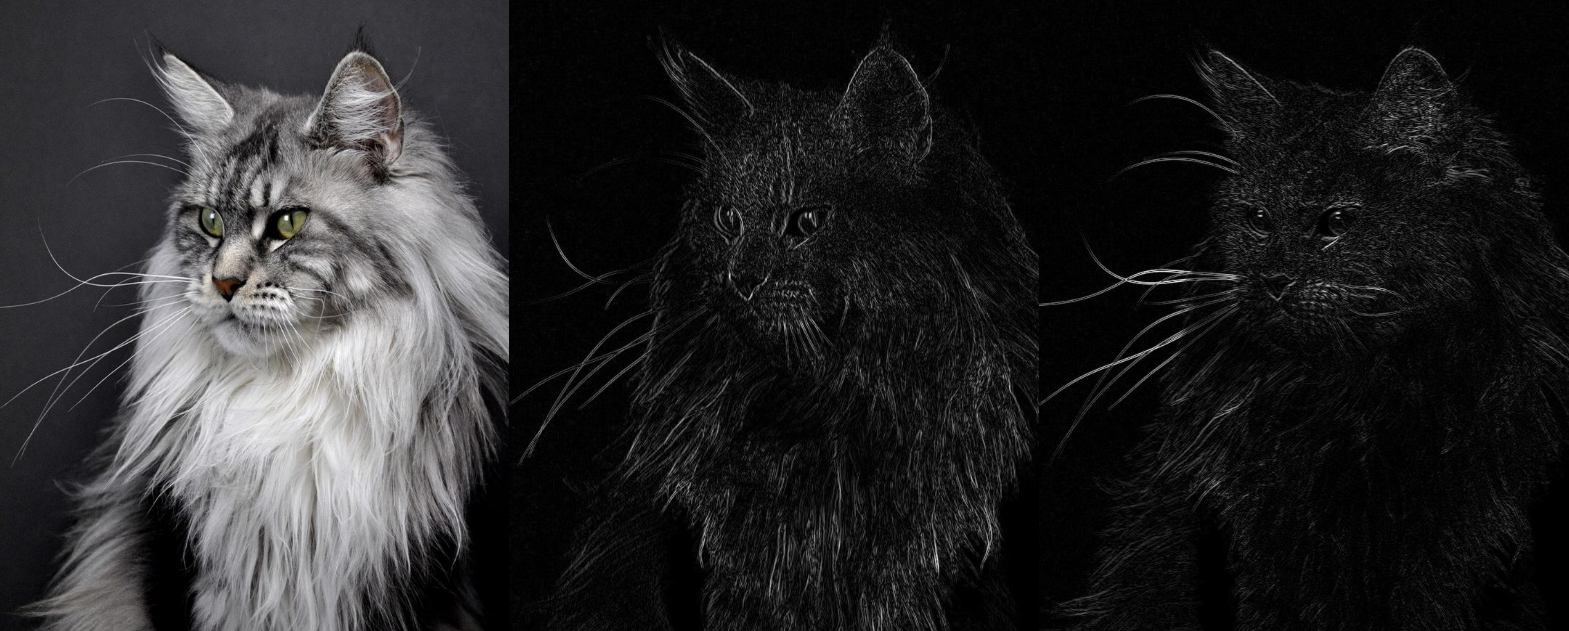
\includegraphics[scale=0.33]{katter.png}
  	\caption{The result of a filter for vertical and horizontal edge detection applied on a picture of a cat.} \label{figkatter}
\end{figure}

In feed-forward neural networks every neuron in a layer is connected to all the neuron in the next layer. If you would use feed-forward neural networks for a computer vision problem you would reshape the given input image to a single $CHW$-dimensional vector where $W$ and $H$ are the images width and height in pixels and $C$ is the number of color channels in the image. Because every neuron in the previous layer is connected to all the neurons in the proceeding layer most of the spatial information in the image is lost. Convolutional neural networks are different in the way how they operate on spatially local data. The neurons in layer $l$ are only connected to the neurons in layer $l+1$ that are in the close spatial vicinity of the neurons in layer $l$. In practice this has yielded more accurate predictions over their feed-forward counterparts and has lead to the model becoming the state of the art in computer vision \cite{cs231n} \cite{convmath} \cite{convarithmetic}.

\subsection{Model structure, parameters and notation}
Convolutional neural networks are composed of a number of layers stacked on top of each other, similar to feed-forward neural networks. The difference between these two models is how one layer is connected to the next layer. While feed-forward neural networks have only one type of layer, convolutional neural networks have a wide variety of different layers. The five elementary layers and operations of the convolutional neural network are the convolutional layer, the maxpooling layer, the softmax layer, the activation function layer and batch normalization, which all behave differently. A convolutional neural network can also use fully connected layers where every neuron in a layer $l$ is connected to all neurons in layer $l+1$, which behave exactly the same as feed-forward neural networks \cite{cs231n} \cite{convmath} \cite{convarithmetic}.

At every layer $l$ there are parameters $\theta^{(l)}$ and activations (neurons) $X^{(l)}$. The last layer is characterized by $\hat{y}$ and $X^{(L)}$ where $L$ is the number of layers in the network. Given an input $X^{(1)}$ the model predicts values $\hat{y}$. The input is forward propagated recursively by using the activations $X^{(l)}$ and parameters $\theta^{(l)}$ from layer $l$ to compute the activations in layer $l+1$, defined by equation \eqref{CNNeq}. Simiar to feed-forward neural network, the prediction is then put into a loss function $L(\theta)$, which is used by the backpropagation algorithm along with Stochastic Gradient Descent to train the network \cite{cs231n} \cite{convmath}.

\begin{equation}\label{CNNeq}
X^{(1)} \xrightarrow{\theta^{(1)}} X^{(2)}  \xrightarrow{\theta^{(2)}} \cdots  \xrightarrow{\theta^{(L-2)}} X^{(L-1)}  \xrightarrow{\theta^{(L-1)}} X^{(L)} = \hat{y}
\end{equation}

To be able to fully utilize the spatial information from a given input the model represent the activation at a given layer $l$ as a tensor of order 4: $X^{(l)} \in \mathbb{R}^{R \times C  \times H \times W}$. A layer takes in a batch of three-dimensional volumes of neurons and produces a new batch of three-dimensional volumes of neurons at the next layer. $R$ stands for the batch size and $C$, $W$ and $H$ are the depth, width and and height of the volume of neurons. To feed an image into the model, the image is made into a tensor of size $3 \times H \times W$ where the values of the neurons are the value of the pixels in the image, for all 3 red, green and blue color channels in the image. The image tensors are then stacked into a single tensor of size $R \times 3 \times H \times W$ to form a mini-batch \cite{cs231n}.

A $H \times W$ slice of the activations is called a feature map or a channel. Convolutional neural networks are usually illustrated as three-dimensional volumes of activations (see figure \ref{figvgg}) or as stacked feature maps (see figure \ref{figboatcnn}) \cite{cs231n} \cite{convmath} \cite{convarithmetic}. 

\begin{figure}[h]
	\centering
  		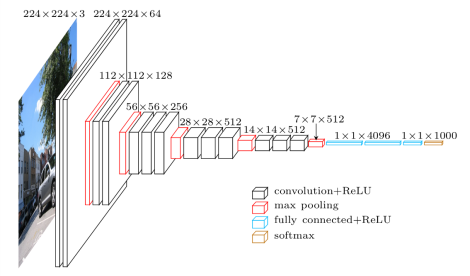
\includegraphics[scale=0.6]{vggnet.png}
  	\caption{An illustration \cite{vgg} of a the VGGNet19 convolutional neural network. The different volumes represent the activations of the network at different depths. Each two-dimensional slice is a feature map.} \label{figvgg}
\end{figure}

\begin{figure}[h]
	\centering
  		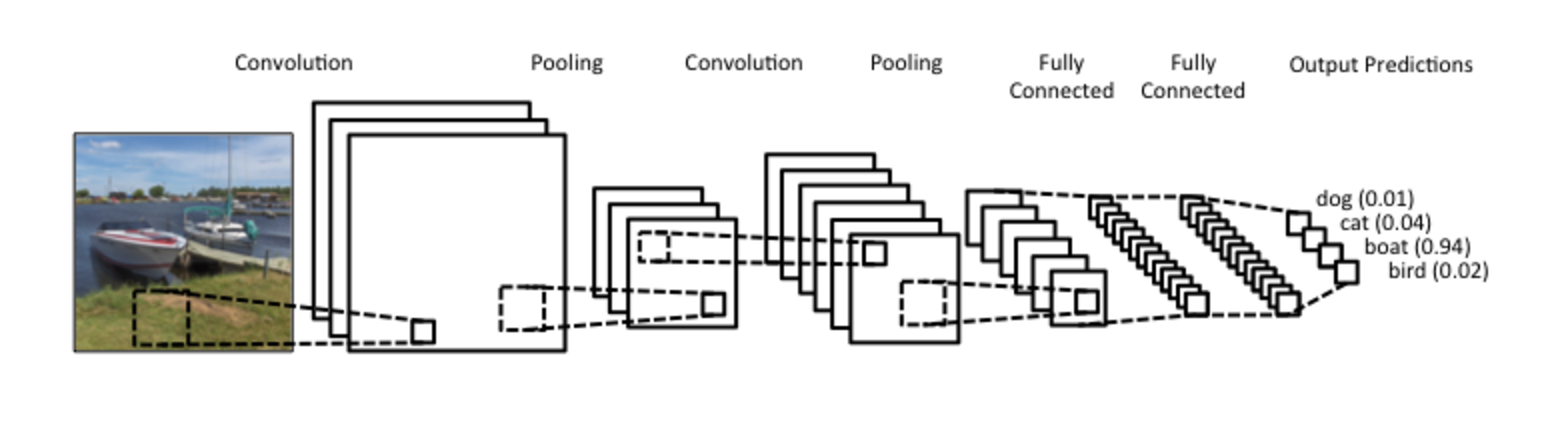
\includegraphics[scale=0.6]{boatcnn.png}
  	\caption{An illustration \cite{figkonv} of a convolutional neural network. Each two-dimensional slice is a feature map.}\label{figboatcnn}
\end{figure}

Every single type of layer in a convolutional neural network has two modes: forward propagation and backpropagation. The model is trained the same way as a feed-forward neural network is trained: A given input is forward propagated to get a loss which is then backpropageted though the network. Thus, for every layer there has to be a definition of forward propagation and backpropagation. In the forward propagation the activations from the previous layer are used to calculate the activations in the next layer. During backpropagation the delta-error from the next layer is used to calculate the delta-error of the previous layer. The delta-error is then used to compute the partial derivatives needed for the gradient \cite{cs231n} \cite{convmath}. 

Because every layer operation in the neural network is defined sequentially, we only have to define operations for two adjacent layers. Let the size of the tensor of activations at layer $l$ have size $R \times C \times H \times W$. At the next layer, $l+1$, the activations will be of size $R \times C' \times H' \times W'$. The prime notation specifies that the variable originates from the proceeding layer and is the same for the indices. The tensors are indexed by the four-tuple $(r, c, h, w)$. The batch size always stays the same from layer to layer, while the spatial size can decrease depending on the layer type \cite{cs231n} \cite{convmath}. 

\subsection{Convolution forward propagation}
The basic building block of the convolutional neural network is the convolution and the convolutional layer. It uses the learnable parameters $W^{(l)} \in \mathbb{R}^{C' \times C  \times k \times k}$, called a kernel, and is the before mentioned filter the network learns to apply to images. $C$ and $C'$ are the number of channels in layer $l$ and $l+1$ respectively. $k$ is a variable called the kernel size of the convolution \cite{cs231n}. 

The activations at layer $l+1$ are derived from the activations at layer $l$ by applying the kernel at every possible spatial location on the activations at layer $l$ (see figure \ref{figkonv}). Every neuron is multiplied by the value of the kernel at the same spatial location. The sum of all the products becomes the activation of a single neuron in layer $l+1$. Applying this operation on every region of neurons in the activation is called a convolution. The convolution operator is denoted by $*$ \cite{cs231n} \cite{convmath} \cite{convarithmetic}. 

\begin{figure}[h]
	\centering
  		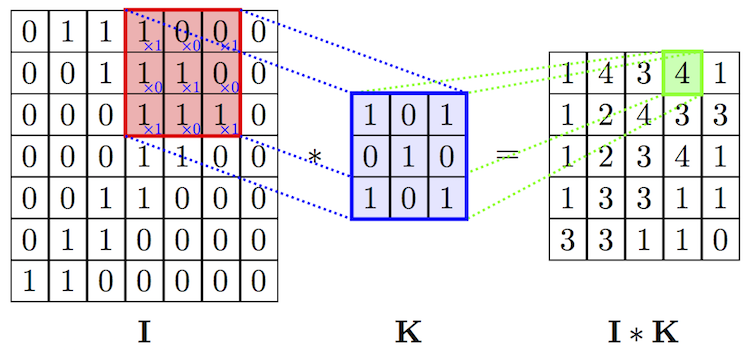
\includegraphics[scale=2.1]{convolution.png}
  	\caption{A kernel of size $1 \times 3 \times 3$ convolving over activations of size $1 \times 7 \times 7$, producing activations of size $1 \times 4 \times 4$ in the next layer \cite{figconv}. } \label{figkonv}
\end{figure}

A feature map in layer $l+1$ is the result of a single kernel of size $1 \times C  \times k\times k$ being convolved over the whole activation volume of the previous layer. $C'$ is the number of kernels a layer has and is also the number of feature maps the next layer will have \cite{cs231n} \cite{convmath}. 

The kernels have two additional non-learnable hyperparameters: a stride $s$ and zero-padding $p$. $s$ is the size of the step the kernel takes when it moves from one spatial location to the next during a convolution. The convolution in figure \ref{figkonv} has a stride of $s = 1$. Zero-padding entails padding the edges of the activation tensor with $p$ zeros (see figure \ref{figzeropad}). Since a convolution decreases the spatial size of the activations of the next layer, zero-padding is a way to control the size of the activations \cite{cs231n} \cite{convmath} \cite{convarithmetic}. 

\begin{figure}[h]
	\centering
  		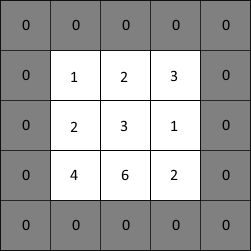
\includegraphics[scale=0.7]{zeropadding.png}
  	\caption{An activation with size $1 \times 3 \times 3$ is zero-padded with $p=1$ and the resulting tensor is of size $1 \times 5 \times 5$. White symbolizes the original tensor and grey symbolizes the padded zeros. } \label{figzeropad}
\end{figure}

Let $W^{(l)} \in \mathbb{R}^{C' \times C  \times k \times k}$, $X^{(l)} \in \mathbb{R}^{R \times C  \times (H+2p) \times (W+2p)}$ and $X^{(l+1)} \in \mathbb{R}^{R \times C'  \times H' \times W'}$. The dimensions of layer $l+1$ are defiend by equations \eqref{eqkonvW} and \eqref{eqkonvH} \cite{cs231n} \cite{convmath} \cite{convarithmetic}: 
\begin{equation}\label{eqkonvW}
W' = \frac{W-k+2p}{s} +1
\end{equation}
\begin{equation}\label{eqkonvH}
H' = \frac{H-k+2p}{s} +1
\end{equation}
The following equation defines the convolutional layer algebraically \cite{cs231n} \cite{convmath}:
\begin{equation}\label{konvolution}
\begin{split}
	\begin{bmatrix} X^{(l+1)} \end{bmatrix}_{r, c', h', w'}	
		& = X^{(l)}_{r, c', h', w'} *W^{(l)}_{c'} \\
		& = \sum^{C-1 }_{c=0} \sum^{k-1 }_{j=0} \sum^{k-1 }_{i=0} X^{(l)}_{r, c, (1+sh'-s+j), (1+sw'-s+i)}W^{(l)}_{c', c, j, i}
\end{split}
\end{equation}

The index of the term which shall be used to convolve specifies which dimensions will be convolved upon and summed over. For instance, $W^{(l)}_{c'}$ implies that the $C$, $H$ and $W$ dimensions (all channels) should be used in the convolution, while $W^{(l)}_{c', c}$ implies that only the $H$ and $W$ dimension (one channel) should undergo the convolution operation.

Convolutions are in practice implemented with the functions $row2im$ and $im2row$ which enable the convolution to be computed with a single dot product \cite{cs231n} \cite{convmath} \cite{convarithmetic}. The underlying math is equivalent with the equations shown in this paper. However, $row2im$ and $im2row$ are outside of the scope of this paper and are left to the reader to research if a more computationally efficient implementation is required. 

\subsection{Convolution backpropagation}
At every layer $l$ the delta-error of the proceeding layer $\delta^{(l+1)}$ has to be backpropagated to create the delta-error at the current layer. $\delta^{(l)}$ is then used to compute the partial derivatives of the loss with respect to the weights $W^{(l)}$ to be used in the gradient \cite{cs231n} \cite{convmath}. 
 
The backpropagation of the recursive delta-error $\delta^{(l+1)}$ is derived by the use of the chain rule. $\delta^{(l+1)} = \inpd{L(\theta)}{X^{(l+1)}}$ is broken up into two smaller partial derivatives $\inpd{L(\theta)}{X^{(l+1)}}$ and $\inpd{X^{(l+1)}}{X^{(l)}}$. Additionally, because more than one single neuron in layer $l$ is responsible for the delta-error at layer $l+1$, all the neurons of layer $l$ have to be summed over, similar to equation \eqref{dLdX_FCC}, \eqref{dLdW_FCC}, and \eqref{dLdb_FCC}. This can be done since the derivative of a sum is equivalent to the sum of the derivatives of each element. $X^{(l+1)}_{r,c',h',w'}$ is then replaced by its definition from equation \eqref{konvolution} \cite{convmath} \cite{webconv1} \cite{webconv2} \cite{webconv3}: 

\begin{equation}\label{konvolutionbackprop}
\begin{split}
	\delta^{(l)}_{r,c,h,w}
		& = \pd{L(\theta)}{X^{(l)}_{r,c,h,w}} \\
		& = \sum^{C' }_{c'=1} \sum^{H' }_{h'=1} \sum^{W' }_{w'=1} \pd{L(\theta)}{X^{(l+1)}_{r,c',h',w'}} \pd{X^{(l+1)}_{r,c',h',w'}}{X^{(l)}_{r,c,h,w}} \\
		& = \sum^{C' }_{c'=1} \sum^{H' }_{h'=1} \sum^{W' }_{w'=1} \delta^{(l+1)}_{r,c',h',w'} \pd{\sum^{C-1 }_{c=0} \sum^{k-1 }_{j=0} \sum^{k-1 }_{i=0} X^{(l)}_{r, c, (1+sh'-s+j), (1+sw'-s+i)}W^{(l+1)}_{c', c, j, i}}{X^{(l)}_{r,c,h,w}}
\end{split}
\end{equation}

Every partial derivative in the most inner sum will be equal to to zero if $X^{(l)}_{r, c, h'+j, w'+i} \neq X^{(l)}_{r,c,h,w}$. Using the substitutions $h = 1+sh'-s+j$ and $w = 1+sw'-s+i$ the three inner sums are cancelled out \cite{webconv1} \cite{webconv2} \cite{webconv3}:

\begin{equation}
\begin{split}
	\delta^{(l)}_{r,c,h,w}
		& = \sum^{C' }_{c'=1} \sum^{H' }_{h'=1} \sum^{W' }_{w'=1} \delta^{(l+1)}_{r,c',h',w'} \pd{\sum^{C-1 }_{c=0} \sum^{k-1 }_{j=0} \sum^{k-1 }_{i=0} X^{(l)}_{r, c, (1+sh'-s+j), (1+sw'-s+i)}W^{(l+1)}_{c', c, j, i}}{X^{(l)}_{r,c,h,w}} \\
		& = \sum^{C' }_{c'=1} \sum^{H' }_{h'=1} \sum^{W' }_{w'=1} \delta^{(l+1)}_{r,c',h',w'} W^{(l+1)}_{c', c, (h+s-1-sh'), (w+s-1-sw')}     \\
\end{split}
\end{equation}


Which one can see is a sum of convolutions (for the special case $s=1$) where a feature map of the delta-error of layer $l+1$ convolves over all the kernels of layer $l$ where the kernels are rotated by $180^\circ$. This is intuitive since every feature map in $X^{(l)}$ is used to create a single feature map in $X^{(l+1)}$.

The partial derivative of the loss $L(\theta)$ with respect to the weights $W^{(l)}$ is derived the same way the backpropagation of the error is derived. Now the $R$-dimension is additionally summed over since the loss is a function of every example in the mini-batch, and affects the gradient \cite{cs231n} \cite{webconv1} \cite{webconv2} \cite{webconv3}. 
\begin{align}
\begin{split}
	\pd{L(\theta)}{W^{(l)}_{c',c,h,w}}
		& = \sum^{R }_{r=1} \sum^{C' }_{c''=1} \sum^{H' }_{h'=1} \sum^{W' }_{w'=1} \pd{L(\theta)}{X^{(l+1)}_{r,c'',h',w'}} \pd{X^{(l+1)}_{r,c'',h',w'}}{W^{(l)}_{c',c,h,w}} \\
		& = \sum^{R }_{r=1} \sum_{c''=1}^{C' } \sum^{H' }_{h'=1} \sum^{W' }_{w'=1} \delta^{(l+1)}_{r,c'',h',w'} \pd{\sum\limits^{C-1 }_{c=0} \sum\limits^{k-1 }_{j=0} \sum\limits^{k-1}_{i=0} X^{(l)}_{r, c, (1+sh'-s+j), (1+sw'-s+i)}W^{(l)}_{c'', c, j, i}}{W^{(l)}_{c',c,h,w}} \\
		& = \sum^{R }_{r=1} \sum^{H' }_{h'=1} \sum^{W' }_{w'=1} X^{(l)}_{r, c, (1+sh'-s+h), (1+sw'-s+w)} \delta^{(l+1)}_{r,c',h',w'} \\
\end{split}
\end{align}

\subsection{Activation function forward propagation}
In the activation function layer an activation function $f$ is applied element wise on every neuron in the activation tensor. Thus, the size of $X^{(l)}$ and $X^{(l+1)}$ is the same. Any differentiable function can be used as an activation function, but the most commonly used ones are ReLU, sigmoid and $\tanh$. The activation function layer does not have any learnable parameters. Activation functions enable the network to learn faster while also increasing the accuracy of the predictions \cite{cs231n} \cite{convmath}. 
 
Forward propagation is defined by:
\begin{equation}\label{eqactivation}
X^{(l+1)}_{r,c,h,w} = f(X^{(l)}_{r,c,h,w})
\end{equation}

\subsection{Activation function backpropagation}
Because the activation function layer does not have any learnable parameters only the recursive delta-error has to be backpropagated. It is derived by the use of the chain rule. $\inpd{L(\theta)}{X^{(l)}}$ is split up into $\inpd{L(\theta)}{X^{(l+1)}}$ and $\inpd{X^{(l+1)}}{X^{(l)}}$. The first term is simply the delta-error of the proceeding layer and the second term is the derivative of the activation function \cite{cs231n} \cite{convmath}: 

\begin{equation}
\begin{split}
\delta^{(l)}_{r,c,h,w}
		& = \pd{L(\theta)}{X^{(l)}_{r,c,h,w}} \\
		& = \pd{L(\theta)}{X^{(l+1)}_{r,c,h,w}} \pd{X^{(l+1)}_{r,c,h,w}}{X^{(l)}_{r,c,h,w}} \\
		& = \delta^{(l+1)}_{r,c,h,w} f'(X^{(l)}_{r,c,h,w})
\end{split}
\end{equation}

\subsection{Maxpooling forward propagation}
Maxpooling is a way to reduce the spatial size of the activations from one layer to the next. Every feature map in layer $l$ is divided into a number of regions of size $k \times k$ where $k$ is the hyperparameter called kernel size. One single $k \times k$ region corresponds to a single activation in the proceeding layer $l+1$. The activation is given by the maximum value of the region (see figure \ref{figmaxpool}). Additionally, maxpooling also has the hyperparameter $s$, called its stride, and works similar to the stride for the convolutional layer. $s$ denotes the step size that the $k \times k$ region uses when it traverses the volume of activations. Maxpooling does not have any learnable parameters \cite{cs231n} \cite{convmath} \cite{convarithmetic}. 

\begin{figure}[h]
	\centering
  		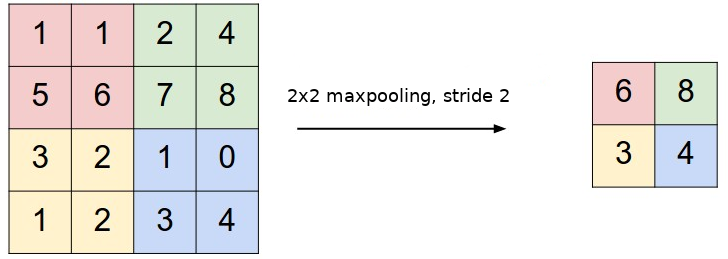
\includegraphics[scale=0.7]{maxpool.png}
  	\caption{Maxpooling with kernel size $k=2$ and stride $s=2$ on an area of size $4 \times 4$. The resulting area has size $2 \times 2$ \cite{figkonv}} \label{figmaxpool}
\end{figure}

Similar to a convolution without zero-padding, the dimensions of the proceeding layer is defined by the following equations. The number of feature maps remain constant \cite{cs231n} \cite{convmath} \cite{convarithmetic}: 
\begin{equation}
W' = \frac{W-k}{s}+1
\end{equation}
\begin{equation}
H' = \frac{H-k}{s}+1
\end{equation}
\begin{equation}
C' = C
\end{equation}

The following equation defines the maxpooling layer algebraically \cite{cs231n} \cite{convmath}:
\begin{equation}\label{maxpool}
X^{(l+1)}_{r,c',h',w'} = \underset{0 \leq j < k, \ 0 \leq i < k}{\max} X^{(l)}_{r,c',(h's+j),(w's+i)}
\end{equation}

\subsection{Maxpooling backpropagation}
Maxpooling does not have any learnable parameters and thus only the recursive delta-error has to be backpropagated. With the use of the chain rule the delta-error at layer $l$ is split into two partial derivatives $\inpd{L(\theta)}{X^{(l+1)}}$ and $\inpd{X^{(l+1)}}{X^{(l)}}$. The first term is the delta-error at layer $l+1$. $X^{(l+1)}$ is then substituted with its definition from equation \eqref{maxpool} \cite{cs231n} \cite{convmath} \cite{webconv3}: 

\begin{equation}
\begin{split}
	\delta^{(l)}_{r,c,h,w}
		& = \pd{L(\theta)}{X^{(l)}_{r,c,h,w}} \\
		& = \pd{L(\theta)}{X^{(l+1)}_{r,c',h',w'}} \pd{X^{(l+1)}_{r,c',h',w'}}{X^{(l)}_{r,c,h,w}} \\
		& = \delta_{r,c',h',w'} \pd{\underset{0 \leq j < k,0 \leq i < k}{\max} X^{(l)}_{r,c',(h's+j),(w's+i)}}{X^{(l)}_{r,c,h,w}} \\
\end{split}
\end{equation}

The partial derivative in the last equation will be equal to 1 if and only if $X^{(l)}_{r,c',(h's+j),(w's+i)} = X^{(l)}_{r,c,h,w}$. For any other case $X^{(l)}_{r,c,h,w}$ will not have any effect on the neurons in the proceeding layer $l+1$ and the partial derivative will thus be equal to 0 \cite{cs231n} \cite{convmath} \cite{webconv3}:
\begin{equation}
\delta^{(l)}_{r,c,h,w} = \begin{cases}
				\delta_{r,c,h',w'} & \mbox{if } \begin{split} h = h's+j, \\w = w's+i \end{split}\\
				0 & \mbox{otherwise}\\
			\end{cases}
\end{equation}

The delta-error from layer $l+1$ is thus redirected to the neuron in layer $l$ that is responsible for the activation which the delta error at layer $l+1$ corresponds to. If a neuron in layer $l$ is responsible for two or more activations in layer $l+1$ its delta error will become the sum of the delta-errors of the activations in question \cite{cs231n} \cite{convmath} \cite{webconv3}. 

\subsection{Batch Normalization forwardpropagation}
Neural networks are hard to train because of their recursive nature. A small change in the weights of the first layer will have a cascading effect throughout the network: The changed second layer will create a slightly larger deviation in the third layer, and the change in the third layer will have an even bigger effect on the fourth layer, and so on. One small change in the first layers can have a dramatic effect on the final prediction of the neural network. This is called  the internal covariate shift in the litterature and is what Batch Normalization (BN) sets out to fix \cite{cs231n} \cite{batchnorm}. 

Batch Normalization normalizes every feature map by dividing the feature map with the variance of the whole mini-batch's variance at the specified feature map, and subtracting the mean of the whole mini-batch's feature map. The cascading effect of a change in the first layer causing a bigger change in the last layers will no longer take place since every layer aims to have a variance of 1 and mean of 0. The internal covatiate shift is thus minimized \cite{cs231n} \cite{batchnorm}. 

To derive the activations at layer $l+1$ the mean and variance of every feature map in layer $l$ has to be computed. Let $\mu_c$ and $\sigma^2_c$ be the mean and variance of the feature map $c$ defined by the following equations \cite{cs231n} \cite{batchnorm}: 
\begin{equation}\label{eqmuc}
\mu_c = \frac{1}{RHW} \sum^{R }_{r=1} \sum^{H }_{h=1} \sum^{W }_{w=1} X^{(l)}_{r,c,h,w}
\end{equation}
\begin{equation}\label{eqsigmac}
\sigma^2_c  = \frac{1}{RHW} \sum^{R }_{r=1} \sum^{H }_{h=1} \sum^{W }_{w=1} ({X^{(l)}_{r,c,h,w} - \mu_c})^2
\end{equation}
Let $\hat{X}$ denote the normalized activations \cite{cs231n} \cite{batchnorm}. It is defined by:
\begin{equation}\label{xhat}
\hat{X}_{r,c,h,w} = (X^{(l)}_{r,c,h,w} - \mu_c){(\sigma^2_c)}^{-\frac{1}{2}}
\end{equation}

The normalized activations are then transformed by an affine transformation with the learnable parameters $\gamma_{c}^{(l)}$ and $\beta_{c}^{(l)}$. They enable the network to undo the normalization from equation \eqref{xhat} if the network deems it will result in more accurate predictions. The final activations at layer $l+1$ is defined by the following equation \cite{cs231n} \cite{batchnorm}:
\begin{equation}\label{eqbn}
X^{(l+1)}_{r,c,h,w} = \gamma_{c}^{(l)} \hat{X}_{r,c,h,w} + \beta_{c}^{(l)}
\end{equation}

When the network is used for predictions outside of the training, also called runtime, the network cannot calculate the needed statistics of the mini-batch to perform forward propagation since a batch size of 1 is usually used at runtime. To combat this, the statistics of the whole training data can be used to approximate the mean and variance of the activations. This can be done for small datasets, but is inpractical for training data with millions of examples. Instead, an exponentially weighted moving average which is updated at every forward propagation can be used to approximate the mean and variance of the whole population \cite{cs231n} \cite{batchnorm}. 

Let $\mu_{EWMA_c}$ and $\sigma^2_{EWMA_c}$ denote the exponentially weighted moving average for the mean and variance of the feature map $c$. Let $\lambda$ be the weight decay term. The moving averages are then defined by the following equations:

\begin{equation}\label{eqewmamu}
\mu_{EWMA_c} \to \lambda \mu_c + (1-\lambda)\mu_{EWMA_c}
\end{equation}
\begin{equation}\label{eqewmasigma}
\sigma^2_{EWMA_c} \to \lambda \sigma^2_c + (1-\lambda)\sigma^2_{EWMA_c}
\end{equation}

\subsection{Batch Normalization backpropagation}
At every layer $l$ the delta-error of the previous layer $\delta^{(l+1)}$ has to be backpropagated to create the delta-error at the current layer. The delta-error is then used to compute the partial derivatives of the loss with respect to the learnable parameters $\gamma_{c}^{(l)}$ and $\beta{c}^{(l)}$ to be used in the gradient. To aid the derivation of the backpropagation the kronecker-delta $I$ is used. The kronecker-delta has the following properties \cite{webBN1} \cite{webBN2}: 
\begin{equation}\label{kroneckerdelta}
I_{i,j} = \begin{cases} 1 & \mbox{if } i = j \\ 0 & \mbox{if } i \neq j  \end{cases}
\end{equation}
\begin{equation}\label{kroneckerdeltaDERIVATIVE}
\pd{a_{j}}{a_i} = I_{i,j}
\end{equation}
\begin{equation}\label{kroneckerdeltaSUM}
\sum_j  a_i  I_{i,j} = a_j
\end{equation}

The backpropagation of the recursive delta-error $\delta^{(l+1)}$ is derived by the use of the chain rule. $\inpd{L(\theta)}{X^{(l)}}$ is broken up into three partial derivatives and the sum of all the neurons is taken, similar to equation \eqref{konvolutionbackprop}. Additionally, the $R$-dimension is summed over since every example in the mini-batch has an effect on a single neuron in proceeding layer \cite{webBN1} \cite{webBN2}. 
\begin{align}\label{BN_delta_error}
\begin{split}
	\delta^{(l)}_{r,c,h,w}
		& = \pd{L(\theta)}{X^{(l)}_{r,c,h,w}} \\
		& = \sum^{R }_{r'=1} \sum^{C' }_{c'=1} \sum^{H' }_{h'=1} \sum^{W' }_{w'=1} \pd{L(\theta)}{X^{(l+1)}_{r',c',h',w'}} \pd{X^{(l+1)}_{r',c',h',w'}}{\hat{X}_{r',c',h',w'}} \pd{\hat{X}_{r',c',h',w'}}{{X}^{(l)}_{r,c,h,w}}\\
\end{split}
\end{align}
$\inpd{L(\theta)}{X^{(l+1)}}$ is the delta-error of the proceeding layer. $\inpd{X^{(l+1)}}{\hat{X}}$ is easily differentiable since equation \eqref{eqbn} is a linear equation \cite{webBN1} \cite{webBN2}.

\begin{equation}\label{BN_dxdxhat}
\begin{split}
	\pd{X^{(l+1)}_{r',c',h',w'}}{\hat{X}_{r',c',h',w'}}
		& = \pd{(\gamma_{c'}^{(l)} \hat{X}_{r',c',h',w'} + \beta_{c'}^{(l)})}{\hat{X}_{r',c',h',w'}} \\
		& =\gamma_{c'}^{(l)}
\end{split}
\end{equation}

The partial derivative of the normalized activations $\hat{X}$ with respect to the activations $X^{(l)}$ is derived by substituting $X^{(l)}$ with its definition from equation \eqref{xhat} and then using the product rule \cite{webBN1} \cite{webBN2}: 
\begin{equation}\label{BN_kedjeregeln}
\begin{split}
\pd{\hat{X}_{r',c',h',w'}}{{X}^{(l)}_{r,c,h,w}} 
	& = \pd{(X^{(l)}_{r',c',h',w'} - \mu_{c'}){(\sigma^2_{c'})}^{-\frac{1}{2}}}{{X}^{(l)}_{r,c,h,w}} \\
	& = {(\sigma^2_{c'})}^{-\frac{1}{2}} \pd{(X^{(l)}_{r',c',h',w'} - \mu_{c'})}{{X}^{(l)}_{r,c,h,w}} - \frac{1}{2}(X^{(l)}_{r',c',h',w'} - \mu_c){(\sigma^2_{c'})}^{-\frac{3}{2}} \pd{\sigma^2_{c'}}{{X}^{(l)}_{r,c,h,w}}
\end{split}
\end{equation}

The derivative of the first factor with respect to the activation is derived by substituting the batch mean $\mu_{c'}$ with its definition from equation \eqref{eqmuc} and then using the kronecker-delta from equations \eqref{kroneckerdelta}, \eqref{kroneckerdeltaDERIVATIVE} and \eqref{kroneckerdeltaSUM} \cite{webBN1} \cite{webBN2}: 
\begin{equation}\label{mu'}
\begin{split}
\pd{(X^{(l)}_{r',c',h',w'} - \mu_{c'})}{{X}^{(l)}_{r,c,h,w}}
	& = \pd{({X^{(l)}_{r',c',h',w'} - \frac{1}{RHW} \sum\limits^{R }_{r''=1} \sum\limits^{H }_{h''=1} \sum\limits^{W }_{w''=1} X^{(l)}_{r'',c',h'',w''}})}{{X}^{(l)}_{r,c,h,w}} \\
	& = I_{r',r} I_{c',c} I_{h',h} I_{w',w} - \frac{1}{RHW} I_{c',c}
\end{split}
\end{equation}

The derivative of the second factor with respect to the activation is found in the same way as the previous equation. The batch variance $\sigma^2_{c'}$ is substituted with its definition from equation \eqref{eqsigmac}. The kronecker-delta is later used together with the chain rule \cite{webBN1} \cite{webBN2}:
\begin{equation}\label{sigma'}
\begin{split}
\pd{\sigma^2_{c'}}{{X}^{(l)}_{r,c,h,w}}
	& = \pd{\frac{1}{RHW} \sum\limits^{R }_{r'=1} \sum\limits^{H }_{h'=1} \sum\limits^{W }_{w'=1} ({X^{(l)}_{r',c',h',w'} - \mu_{c'}})^2}{{X}^{(l)}_{r,c,h,w}} \\
	& = \frac{1}{RHW} \sum\limits^{R }_{r'=1} \sum\limits^{H }_{h'=1} \sum\limits^{W }_{w'=1} 2 ({X^{(l)}_{r',c',h',w'} - \mu_{c'}}) (I_{r',r} I_{c',c} I_{h',h} I_{w',w} - \frac{1}{RHW} I_{c',c}) \\
	& = \frac{2}{RHW} ({X^{(l)}_{r,c',h,w} - \mu_{c'}})I_{c',c} - \frac{2}{(RHW)^2}  \sum\limits^{R }_{r'=1} \sum\limits^{H }_{h'=1} \sum\limits^{W }_{w'=1} ({X^{(l)}_{r',c,h',w'} - \mu_{c}}) \\
	& = \frac{2}{RHW} ({X^{(l)}_{r,c',h,w} - \mu_{c'}})I_{c',c}
\end{split}
\end{equation}
The last sum in equation \eqref{sigma'} is equal to zero since it is sums up to be equal to the mean minus the mean.

Equations \eqref{BN_dxdxhat} to \eqref{sigma'} are then substituted into equation \eqref{BN_delta_error} and simplified to form the final expression of the backpropagated delta-error:

\begin{equation}\label{finalBNeq}
\begin{split}
	\delta^{(l)}_{r,c,h,w} 
	& = \sum^{R }_{r'=1} \sum^{C' }_{c'=1} \sum^{H' }_{h'=1} \sum^{W' }_{w'=1} \pd{L(\theta)}{X^{(l+1)}_{r',c',h',w'}} \pd{X^{(l+1)}_{r',c',h',w'}}{\hat{X}_{r',c',h',w'}} \pd{\hat{X}_{r',c',h',w'}}{{X}^{(l)}_{r,c,h,w}}\\
	& = \sum\limits_{r',c',h',w'}\delta^{(l+1)}_{r',c',h',w'} \gamma^{(l)}_{c'} {(\sigma^2_{c'})}^{-\frac{1}{2}} (I_{r',r} I_{c',c} I_{h',h} I_{w',w} - \frac{1}{RHW} I_{c',c}) \\
	& \qquad -\sum\limits_{r',c',h',w'}\delta^{(l+1)}_{r',c',h',w'} \gamma^{(l)}_{c'} \frac{1}{RHW} ({X^{(l)}_{r',c',h',w'} - \mu_{c'}})({X^{(l)}_{r,c',h,w} - \mu_{c'}}) {(\sigma^2_{c'})}^{-\frac{3}{2}} I_{c',c} \\
	& = \delta^{(l+1)}_{r,c,h,w} \gamma^{(l)}_{c} {(\sigma^2_{c})}^{-\frac{1}{2}} - \frac{1}{RHW} \sum\limits_{r',h',w'} \delta^{(l+1)}_{r',c,h',w'} \gamma^{(l)}_{c} {(\sigma^2_{c})}^{-\frac{1}{2}}\\
	& \qquad - \frac{1}{RHW} \sum\limits_{r',h',w'} \delta^{(l+1)}_{r',c,h',w'}\gamma^{(l)}_{c} ({X^{(l)}_{r',c,h',w'} - \mu_{c'}})({X^{(l)}_{r,c,h,w} - \mu_{c}}){(\sigma^2_{c})}^{-\frac{3}{2}} \\
	& = \frac{1}{RHW} \gamma^{(l)}_c {(\sigma^2_{c})}^{-\frac{1}{2}} \biggl(    RHW \delta^{(l+1)}_{r,c,h,w} -  \sum\limits_{r',h',w'} \delta^{(l+1)}_{r',c,h',w'} \qquad \\
	& \qquad -  ({X^{(l)}_{r,c,h,w} - \mu_{c}}) {(\sigma^2_{c})}^{-\frac{3}{2}} \sum\limits_{r',h',w'} \delta^{(l+1)}_{r',c,h',w'} ({X^{(l)}_{r',c,h',w'} - \mu_{c'}}) \biggl) \\
\end{split}
\end{equation}

The derivation of the derivatives of the loss with respect to the parameters are straight-forward and found in a similar way as equation \eqref{BN_delta_error} to \eqref{finalBNeq} \cite{webBN1} \cite{webBN2}. 
\begin{align}
\begin{split}
	\pd{L(\theta)}{\gamma^{(l)}_{c}}
		& = \sum^{R }_{r} \sum^{C' }_{c'} \sum^{H' }_{h'} \sum^{W' }_{w'} \pd{L(\theta)}{X^{(l+1)}_{r,c',h',w'}} \pd{X^{(l+1)}_{r,c',h',w'}}{\gamma^{(l)}_{c}} \\
		& = \sum^{R }_{r} \sum^{C' }_{c'} \sum^{H' }_{h'} \sum^{W' }_{w'} \delta^{(l+1)}_{r,c',h',w'}  \pd{({\gamma_{c'}^{(l)} \hat{X}_{r,c',h',w'} + \beta_{c'}^{(l)}})}{\gamma^{(l)}_{c}} \\
		& = \sum^{R }_{r} \sum^{C' }_{c'} \sum^{H' }_{h'} \sum^{W' }_{w'} \delta^{(l+1)}_{r,c',h',w'} \hat{X}_{r,c,h',w'} I_{c',c}\\
		& = \sum^{R }_{r} \sum^{H' }_{h'} \sum^{W' }_{w'} \delta^{(l+1)}_{r,c,h',w'} \hat{X}_{r,c,h',w'} \\
\end{split}
\end{align}


\begin{align}
\begin{split}
	\pd{L(\theta)}{\beta^{(l)}_{c}}
		& = \sum^{R }_{r} \sum^{C' }_{c'} \sum^{H' }_{h'} \sum^{W' }_{w'} \pd{L(\theta)}{X^{(l+1)}_{r,c',h',w'}} \pd{X^{(l+1)}_{r,c',h',w'}}{\beta^{(l)}_{c}} \\
		& = \sum^{R }_{r} \sum^{C' }_{c'} \sum^{H' }_{h'} \sum^{W' }_{w'} \delta^{(l+1)}_{r,c',h',w'}  \pd{({\gamma_{c'}^{(l)} \hat{X}_{r,c',h',w'} + \beta_{c'}^{(l)}})}{\beta^{(l)}_{c}} \\
		& = \sum^{R }_{r} \sum^{C' }_{c'} \sum^{H' }_{h'} \sum^{W' }_{w'} \delta^{(l+1)}_{r,c,h',w'} I_{c',c}\\
		& = \sum^{R }_{r} \sum^{H' }_{h'} \sum^{W' }_{w'} \delta^{(l+1)}_{r,c,h',w'} \\
\end{split}
\end{align}

\subsection{Softmax forward propagation}
Softmax is used in the last layer of a neural network to bound the predicted values to the interval [0, 1]. It has the properties that the sum of every training example in the mini-batch equals to 1. The activations of the softmax layer can therefore be interpreted as probabilities. If the model wants to classify a given input into one of $C$ classes, the output $\hat{y}$ can be interpreted as the the probability that the given input is of class $c$; $1 \leq c \leq C$, for every class prediction in the output vector \cite{cs231n}.

The input to the softmax layer is resized to a tensor of order 2 $X^{(l)} \in \mathbb{R}^{R \times C}$ and produces an output of the same size. Softmax is defined by the following equation \cite{cs231n}:

\begin{equation}\label{softmax}
\begin{split}
X^{(l+1)}_{r,c}
	& = \dfrac{e^{X^{(l)}_{r,c}}}{\sum^{C }_{c'=1}e^{X^{(l)}_{r,c'}}} \\
\end{split}
\end{equation}

\subsection{Softmax backpropagation}
The softmax layer does not have any learnable parameters and therefore only the recursive delta-error has to be backpropagated. The backpropagation of the recursive delta-error $\delta^{(l+1)}$ is derived by the use of the chain rule. $\inpd{L(\theta)}{X^{(l)}}$ is broken up into the two partial derivatives $\inpd{L(\theta)}{X^{(l+1)}}$ and $\inpd{X^{(l+1)}}{X^{(l)}}$ and the sum of all the neurons in the mini-batch is taken, similar to equations \eqref{konvolutionbackprop} and \eqref{BN_delta_error}. $X^{(l+1)}$ is then substituted with its definition from equation \eqref{softmax} and is differentiated with the product rule and the kronecker-delta. The equation is then simplified with the use of basic algebra \cite{cs231n} \cite{notesonbackprop} \cite{websoftmax}: 
\begin{equation}
\begin{split}
\delta^{(l)}_{r,c}
		& = \pd{L(\theta)}{X^{(l)}_{r,c}} \\
		& = \sum^{C }_{c'=1} \pd{L(\theta)}{X^{(l+1)}_{r,c'}} \pd{X^{(l+1)}_{r,c'}}{X^{(l)}_{r,c}} \\
		& = \sum^{C }_{c'=1} \delta^{(l+1)}_{r,c} \left(  \dfrac{(e^{X^{(l+1)}_{r,c'}})I_{c',c}}{\sum^{C }_{c''=1}e^{X^{(l+1)}_{r,c''}}} - \dfrac{(e^{X^{(l+1)}_{r,c'}})(e^{X^{(l+1)}_{r,c}})}{(\sum^{C }_{c''=1}e^{X^{(l+1)}_{r,c''}})^2} \right) \\
		& = \sum^{C }_{c'=1}  \delta^{(l+1)}_{r,c} X^{(l+1)}_{r,c'}(I_{c',c}-X^{(l+1)}_{r,c}) \\
		& = \delta^{(l+1)}_{r,c} X^{(l+1)}_{r,c} \left( 1-\sum^{C }_{c'=1} X^{(l+1)}_{r,c'} \right)
\end{split}
\end{equation}

\section{Evaluating the models on handwritten digits}
The code and the trained models from this following section are publically available on github in the repository \textit{FCC-vs-CNN-mnist}.

\subsection{MNIST}
The MNIST database for handwritten digits \cite{MNIST} is a dataset consisting of 70 000 grayscale images of size $28 \times 28$ pixels, of the digits 0 to 9 (see figure \ref{figMNIST}). The database is split up into two different sets, a training set containing 60 000 images used to train the model, and a test set consisting of 10 000 images used to evaluate the model. The test set is kept separate from the training set to prevent overfitting on the training data. A model is given all the pixel values of the image as input features, and is asked to predict what digit is in the image.

\begin{figure}[h]
	\centering
  		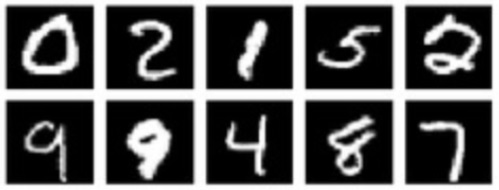
\includegraphics[scale=1]{mnist.png}
  	\caption{Ten images of handwritten digits from the MNIST dataset. \cite{MNIST}} \label{figMNIST}
\end{figure}

\subsection{Method}
A machine learning model can learn to predict what class an object belongs to, from a number of input features, by predicting a $C$-dimensional probability vector $\hat{y}$, where $C$ is the number of object classes to predict. The element $\hat{y}_c$ is the probability that the input to the model is of class $c$, $1 \leq c \leq C$. For neural networks, the probability tensor is a tensor of order 2, $\hat{y} \in \mathbb{R}^{R \times C}$, where $R$ is the batch size and $C$ is the number of object classes.

Let $L(\theta)$ be the loss function used for the classification task. The model is trained by minimizing the cross entropy function which acts on two probability distributions: the predicted probabilities $\hat{y}$ and the real probabilities $y$. Cross entropy and its partial derivative with respect to the last layer of neurons is defined by the following equations \cite{cs231n} \cite{notesonbackprop}: 
\begin{equation}\label{crossentropy}
L(\theta) = - \sum^{R }_{r=1} \sum^{C }_{c=1}y_{r,c} \ \log{\hat{y}_{r,c}}
\end{equation}
\begin{equation}\label{dydxcrossentropy}
\pd{L(\theta)}{\hat{y}_{r,c}} = - \frac{y_{r,c}}{\hat{y}_{r,c}}
\end{equation}

\subsubsection{Models}
Two models were compared on the task of classifying handwritten digits, namely a convolutional neural network and a feed-forward neural network. Table \ref{tabCNN} and \ref{tabFCC} show the network architectures which were chosen on the basis to be as simple as possible, and to have approximately the same number of learnable parameters. The feed-forward model consists of 6 sequential hidden layers of size 128 with ReLU activations, except the last layer which has size $C=10$, and uses a softmax activation. The convolutional model consists of a combination of $3 \times 3$ convolutions with stride 1, 64 channels and 0 zero-padding, and $2 \times 2$ maxpooling layers with stride 2. Every convolutional layer is preceeded by Batch Normalization (BN), and proceeded by a ReLU activation layer, except the last layer which uses a softmax activation. Both network's outputs are interpreted as probabilities that the image is of one of $C$ classes. The network architectures are shown in tables \ref{tabCNN} and \ref{tabFCC}.

\begin{table}[h]
\begin{center}
    \begin{tabular}{c | c | c | c}
    Layer & Kernel Size & Stride & Activation Size \\ 
    \hline \hline
    Input &  &  & $R \times 1 \times 28 \times 28$  \\ 
    BN + Convolution + ReLU & 3 & 1 & $R \times 64 \times 26 \times 26$  \\
    BN + Convolution + ReLU & 3 & 1 & $R \times 64 \times 24 \times 24$  \\ 
    Maxpooling & 2 & 2 & $R \times 64 \times 12 \times 12$  \\ 
    BN + Convolution + ReLU & 3 & 1 & $R \times 64 \times 10 \times 10$  \\ 
    BN + Convolution + ReLU & 3 & 1 & $R \times 64 \times 8 \times 8$  \\ 
    BN + Convolution + ReLU & 3 & 1 & $R \times 64 \times 6 \times 6$  \\
    Maxpooling & 2 & 2 & $R \times 64 \times 3 \times 3$  \\
    BN + Convolution + ReLU & 3 & 1 & $R \times 10 \times 1 \times 1$  \\
    Softmax &  &  & $R \times 10$  \\
    \end{tabular}\caption{\textbf{Convolutional model architecture.} The convolutional neural network used in the experiments. Here R is the batch size.}\label{tabCNN}
\end{center}
\end{table}
\begin{table}[h]
\begin{center}
    \begin{tabular}{c | c | c }
    Layer & Hidden Size & Activation Size \\ 
    \hline \hline
    Input &  &  $R  \times 784$  \\ 
    BN + Fully Connected + ReLU & 128  & $R \times 128$  \\
    BN + Fully Connected + ReLU & 128  & $R \times 128$  \\
    BN + Fully Connected + ReLU & 128  & $R \times 128$  \\
    BN + Fully Connected + ReLU & 128  & $R \times 128$  \\
    BN + Fully Connected + ReLU & 128  & $R \times 128$  \\
    BN + Fully Connected + ReLU & 10  & $R \times 10$  \\
    Softmax &  &  $R \times 10$  \\
    \end{tabular}\caption{\textbf{Feed-forward model architecture.} The feed-forward neural network used in the experiments. Here R is the batch size. Hidden size is the number of neurons in the feed-forward layer.}\label{tabFCC}
\end{center}
\end{table}

\subsection{Results}
The models were trained on a subset of the training set. 5 000 random samples from the training set were chosen as a validation set to track while training the model. The remaining 55 000 images of the training set were used to train the neural networks through SGD with a momentum \cite{cs231n} of 0.9.

For my own implementation of both convolutional neural networks and feed-forward neural networks, the models were trained on an Intel i7 3770K CPU for 5 000 iterations with a learning rate of 0.001 and a batch size of 50. The total elapsed training time was 6 hours per model. The convolutional and feed-forward models achieved a final accuracy of 99.1\% and 97.0\% respectively on the test set of never before seen handwritten digits. 

My own implementations of artificial neural network was deemed to be too computationally inefficient to do any further testing on, so I implemented the models in Facebook's GPU-accelerated tensor and dynamic neural network library PyTorch.

The models were trained for 100 000 iterations while tracking the training and validation loss simultaneously, shown in figure \ref{figaccloss}. The initial learning rate was set to 0.001 and divided by 10 at 70 000 and 90 000 iterations. An Nvidia GTX 1080ti GPU was used to train the models. The models weights were saved every 5 000 iterations. The weights which performed best on the validation set were picked and used to compute the final results on the test set. Results are shown in table \ref{tablemnist}.

\begin{figure}[h]
    \centering
    \subfloat[Accuracy]{{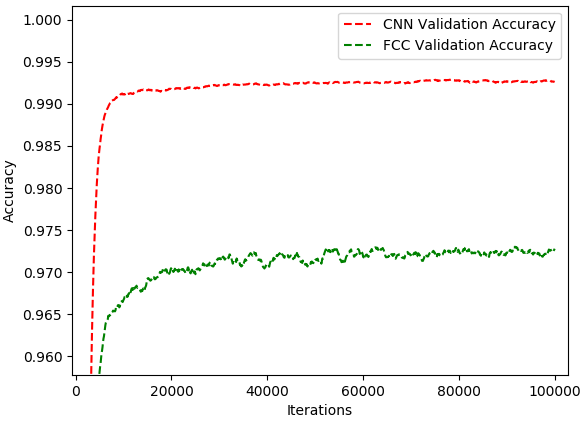
\includegraphics[width=8cm]{accuracy.png} }}
    \subfloat[Losses]{{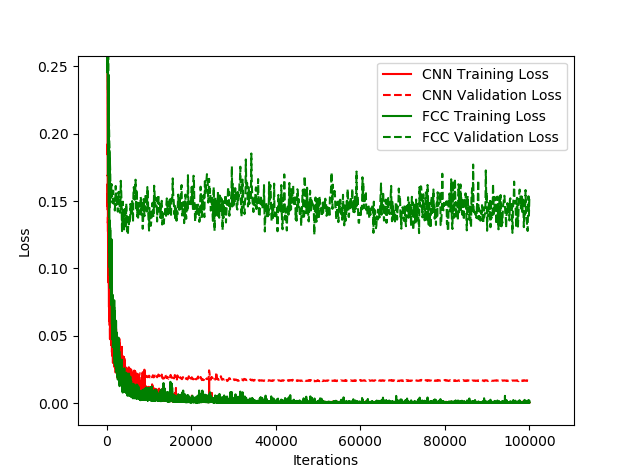
\includegraphics[width=8cm]{losses.png} }}
    \caption{The accuracy (a) and loss (b) of the convolutional model (CNN) and the feed-forward model (FCC) as a function of the numbers of iterations trained. The training loss is the loss on the training set and the validation loss is the loss on the test set. Accuracy is measured on the test set.} \label{figaccloss}
    
\end{figure}
\begin{table}[h]
\begin{center}
    \begin{tabular}{| l | l | l | l | l | l |}
    \hline
    Model & Test Accuracy & Validation Loss & Training Loss & Parameters\\ \hline
    Feed-forward Neural Network & 97.40\% & 0.146 & 0.0010 & 167 168 \\ \hline
    Convolutional Neural Network & 99.30\% & 0.026 & 0.0003 & 153 792\\ \hline
    \end{tabular}
    \caption{The final accuracy and validation loss of the models. The accuracy is measured as the percentage of correctly classified examples from the test set of 10 000 never before seen images of handwritten digits. The validation loss is the loss on the test set.} \label{tablemnist}
\end{center}
\end{table}

\subsection{Discussion}

The convolutional neural network is shown to have better generalizability on the test set than its feed-forward counterpart: While the number of parameters and training loss is approximately the same for both the convolutional and feed-forward models, the validation loss is approximately 7 times higher for the feed-forward model. The final accuracy of the two networks were 99.30\% for the convolutional neural network and 97.40\% for the feed-forward neural network, tested on the test set consisting of 10 000 handwritten digits. 


\section{Dense face detection and localization}
In this section I systematically and empirically investigate how to construct and improve a convolutional-neural-network-based model to detect a variable number of faces in an image. Every factor and suggestion which affects the model performance is evaluated one by one and added to a baseline model.

\subsection{WIDERFace}
For the task of detecting a variable number of faces in an iamge, the WIDERFace dataset \cite{WIDERFace} was used. It is a dataset consisting of 32 203 images of a total of 393 703 number of faces at different scales, lighting and occlusions. Every training example consists of a number of bounding boxes which describes all the faces in the image. A bounding box consists of four coordinates specifying its location: two for the upper left corner and two for the bottom right corner of the bounding box. The images are labeled by humans and is called the ground truth of the image.

\subsection{One-shot detectors}
One-shot detectors were first introduced by the model YOLO \cite{yolo} and later modified and improved by the models SSD \cite{ssd}, YOLO9000 \cite{yolo9000}, DSSD \cite{dssd} and RetinaNet \cite{retinanet}. A one-shot detector works by predicting up to tens of thousands of bounding boxes in different spatial positions in an image, that sets out to detect every object in that image. For every set of predetermined spatial positions in the image, the model predicts 4 bounding box coordinates and probability scores that there exists an object inside the specified bounding box.

The model is trained by assigning every bounding box either a negative or a positive label during training, depending on if the bounding box contains a ground truth object or not. A bounding box is said to contain an object if the intersection over union (IoU) \cite{iou} of the area of the bounding box and the area of the ground truth is bigger or equal to a threshold value (0.55). The intersection over union is used to determine how similar two sets $A$ and $B$ are (see figure \ref{figiou}). It is bounded by the interval $[0,1]$ and is defined by the following equation: 

\begin{equation}\label{eqiou}
IoU(A, B)=\frac{|A \cap B|}{|A \cup B|}
\end{equation}

\begin{figure}[h]
	\centering
  		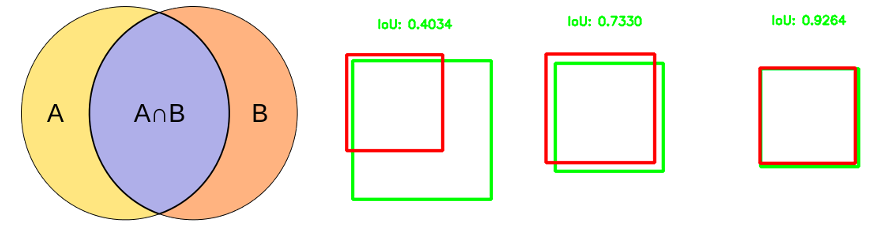
\includegraphics[scale=0.5]{iou.png}
  	\caption{IoU \cite{iou} is defined as the size of the union divided by the size of the intersection of two sets $A$ and $B$. A bigger IoU implies that the predicted bounding box is closer to the ground truth. } \label{figiou}
\end{figure}

\subsection{Baseline model}
The baseline model uses the deep residual convolutional neural network ResNet-18 \cite{resnet} as a backbone network and feature extractor. It uses a total of 18 convolutional layers throughout blocks named \textit{conv1} to \textit{conv5} to extract features from the input image. An additional \textit{conv6} block is created after the last layer to create one additional scale of feature maps. The block consists of one convolutional layer with stride 2, and 2 residual bottleneck layers used by Resnet-50 up to ResNet-152. The feature maps created by the backbone model is then fed into two smaller sub-networks, called the classification head and the regression head. They are constructed out of 4 residual bottleneck layers.

Bounding boxes are created from a number of anchor boxes at every spatial position (width and height) from a set of feature maps. An anchor box is a bounding box of a specific size and scale, used to base the bounding box predictions off. Anchor boxes used by FaceNet are set to be of sizes in the range $[16, 406]$ pixels, each increasing by a factor of $2^{1/3}$ for every new anchor box size. Two ratios of width:height are used at every scale, namely $1:\frac{2}{3}$ and $1:1$, to enable the detection of faces facing sideways and directly into the camera. having densely packed anchors makes it that every ground truth bounding box (of sufficient size) has an IoU$>0.55$ with at least one anchor box. The anchor boxes are spaced out to include 3 scales with 2 aspect ratios across feature maps from the levels \textit{conv2} to \textit{conv5}, to enable the detection of faces of different scales, similar to RetinaNet \cite{retinanet}.

The regression and classification sub-networks take in the last convolutional output from a single network level (\textit{conv2} to \textit{conv5}) as input. Let $W$ and $H$ be the width and height of the tensor of activations at a single network level, and $C$ be the amount of classes to classify. FaceNet uses $C=2$, one for a background class (no face) and one for a foreground class (a face). The classification head predicts $C$ probabilities for every anchor $A$, that there exists a face in the anchor box at every spatial location ($W \times H$), for a total of $KWHA$ values. The regression head predicts $4$ coordinate offsets for every point of the anchor box, for it to match the ground truth as closely as possible, for a total of $4WHA$ coordinate offsets. Additionally, similar to RetinaNet \cite{retinanet}, the last conventional layer which predicts class probabilities uses a bias $b = -\log{\frac{C(1-\pi)}{\pi}}$, such that the model, when first initialized, predicts a probability of $\pi$ for the case of there existing a foreground class (a face) in every bounding box. $\pi = 0.001$ was used.

If not otherwise stated, each version of FaceNet is trained for 70 000 iterations on an Nvidia GTX 1080ti with an initial learning rate of 0.0001, and lowering the learning rate by a factor of 10 after 50 000 and 60 000 iterations. Due to memory limitations a batch size of 8 is used. The models are trained on square image crops, randomly picked to be of between 0.33 and 0.95 of the short size of the image, and resized to be of size $512^2$ pixels. This is done to artificially increase the size of the training data. Additionally, the image is flipped horizontally with a probability of 0.5.

The models are evaluated on the WIDERFace validation set, using the easy, medium and hard splits provided by the WIDERFace evaluation server. The evaluation metric is mean average precision (mAP), and is the area under the precision-recall curve, when plotting the models precision as a function of the recall.

\subsubsection{v1.0, Cross Entropy (CE)}
The first loss function tested is a sum of a coordinate regression loss $L_r$, and a bounding box classification loss $L_c$. $L_r$ is the Smooth L1 Loss \cite{cs231n} and $L_c$ is the softmax cross entropy loss (CE).

The total loss $L(\theta)$ is the mean of the regression losses $L_r$ of all positively assigned anchors plus the mean of the classification losses of all anchors. Negatively assigned anchors do not have any effect on the regression loss. Let $r_a$ and $\hat{r}_a$ be the predicted and ground truth coordinate offsets for anchor box $a$. Let $p_a$ and $\hat{p}_a$ be the predicted and ground truth probability score respectively, for anchor $a$ to contain a face. Let $N$ be the set containing all anchor boxes $a$, and $N_{pos}$ be the set containing every positively assigned anchor box. The total loss is defined as:

\begin{equation}\label{eqfocalloss}
L_r(x) = \begin{cases}
				0.5x^2 & \mbox{if } |x| < 1\\
				|x| - 0.5 & \mbox{otherwise}\\
			\end{cases}
\end{equation}

\begin{equation}\label{eqsmoothl1loss}
L_c(p, \hat{p}) = -p \log{\hat{p}}
\end{equation}



\begin{equation}
\begin{split}
	L(\theta) = &  \frac{1}{|N|} \sum_{a \in N} L_c(p_a, \hat{p}_a) 
	 + \frac{1}{|N_{pos}|} \sum_{a \in N_{pos}} L_r(r_a - \hat{r}_a)  \\ 
\end{split}
\end{equation}

When evaluated on the WIDERFace validation set, the model achieved an mAP of 0 across all 3 sets: easy, medium and hard. The model converged to classify every single bounding box as a negative example, resulting in no faces being found in any image.

\subsubsection{v1.1, Binary Cross Entropy (BCE)}
The baseline model uses a softmax function to base its classification prediction on, based on two values; one for each object class. An open source implementation of YOLO \cite{sigmoidvssoftmax} showed that using a binary cross entropy loss function (logistic regression), instead of a categorical cross entropy using a softmax function, led to a gain in mAP. For FaceNet v1.1, the softmax layer in FaceNet is replaced by a sigmoid function, and logistic regression is used instead. Let the new classification loss be denoted by $L_c$. Instead of normalizing the loss by the total number of bounding boxes, the loss is divided by the total number of positively assigned bounding boxes, similar to SSD \cite{ssd} and RetinaNet \cite{retinanet}.

\begin{equation}
L_c(p, \hat{p}) = -p \log{(\hat{p})} -(1-p) \log{(1-\hat{p})}
\end{equation}

\begin{equation}
\begin{split}
	L(\theta) = &  \frac{1}{|N_{pos}|} \sum_{a \in N} L_c(p_a, \hat{p}_a) 
	 + \frac{1}{|N_{pos}|} \sum_{a \in N_{pos}} L_r(r_a - \hat{r}_a)  \\ 
\end{split}
\end{equation}

When evaluated on the easy/medium/hard splits of the WIDERFace validation set, FaceNet v1.1 achieves an mAP of 37.4/21.7/9.7. 

\subsubsection{v1.2, Focal Loss (FL)}
Focal loss, introduced by RetinaNet \cite{retinanet}, introduced a loss function which focused on the examples which were hard to classify. It was showed that using focal loss instead of cross entropy for multi-class object detection increased the final accuracy of the model. Let $F_c$ denote the focal loss used as the classification loss by FaceNet v1.2:

\begin{equation}
L_c(p, \hat{p}) = -p (1-p)^\gamma \log{(\hat{p})} -(1-p) p^\gamma\log{(1-\hat{p})}
\end{equation}

Since FaceNet proposes a larger number of bounding boxes compared to RetinaNet, a $\gamma$ value of 3 was used, instead 2 used by RetinaNet, to offset the increase in bounding boxes. The total loss $L(\theta)$ is defined by:

\begin{equation}
\begin{split}
	L(\theta) = &  \frac{1}{|N_{pos}|} \sum_{a \in N} L_c(p_a, \hat{p}_a) 
	 + \frac{1}{|N_{pos}|} \sum_{a \in N_{pos}} L_r(r_a - \hat{r}_a)  \\ 
\end{split}
\end{equation}

Using the focal loss instead of binary cross entropy led to an average 10 point decrease in mAP in every category. The results of the easy/medium/hard splits were 22.4/12.1/5.1.

\subsubsection{v1.3, FPN, BCE}
Using a feature pyramid network (FPN) together with a standard backbone ResNet network has been shown to yield higher detection and classification accuracies \cite{fpn}. Instead of only basing the face predictions of the feature maps from $conv2$ to $conv6$ of the backbone network, a top-down architecture from the FPN is used to enable the feature maps at lower scales to make use of higher level features. The same binary cross entropy function of FaceNet v1.1, which performed best, was used.

Adding an FPN to FaceNet yielded a dramatical increase in mAP: The results on the easy/medium/hard splits were 89.3/85.9/65.9, a 1200\% increase in mAP on the hard set.

\subsubsection{v1.4, FPN, FL}
The focal loss is evaluated once again, but with the addition of a feature pyramid network. Everything but the classification loss is kept the same from FaceNet v1.4. The loss function from FaceNet v1.2 is used.

The results on the easy/medium/hard splits were 81.0/81.0/64.2 mAP. Focal loss performed worse than binary cross entropy, when all other factors and hyperparameters were kept the same.

\subsubsection{v1.5, FPN, BCE, level}
The loss function was modified once again to study the effects it had on the accuracy. Instead of normalizing all the losses by the total number of positively assigned anchors, each classification and regression loss is computed separately at every pyramid level. Let $P$ be the set of all pyramid levels $p$, $N^p$ be the set of all created anchor boxes at every spatial position at pyramid level $p$, and $N^p_{pos}$ be the set of all positively assigned anchors at pyramid level $p$. The total loss $L(\theta)$ is defined by:

\begin{equation}
\begin{split}
	L(\theta) = & \sum_{p \in P} \frac{1}{|N^p_{pos}|} \sum_{a \in N^p} L_c(p_a, \hat{p}_a) \\
	 & + \sum_{p \in P}  \frac{1}{|N^p_{pos}|} \sum_{a \in N^p_{pos}} L_r(r_a - \hat{r}_a)  \\ 
\end{split}
\end{equation}

The level separated loss performed slightly worse than the previous non-level-specific version. The results on the easy/medium/hard set were 87.2/82.5/50.4 mAP.

\subsubsection{v1.6, FPN, FL, level}
The loss function from FaceNet v1.5 was used, but replacing the binary cross entropy loss with the focal loss. This resulted in a worse performing model: A decrease of approximately 2 mAP, compared to the binary cross entropy level separated loss. 

The model achieved an mAP of 85.1/80.0/50.6 on the easy/medium/hard splits, performing worse on the easy and medium split, but performing better on the hard split, compared to the binary cross entropy loss.

\subsubsection{v1.7, OHEM, single image}
Online hard example mining (OHEM) \cite{ohem} has been shown to increase mAP when training region based object detectors. Models using OHEM only train on the top $k$ bounding box classification losses, after non-maxima supression (NMS) is applied, in an effort to balance the ratio of negative to positive bounding boxes. Since FaceNet predicts 250 000 bounding boxes for an image of size $512^2$ pixels, the ratio of negatively to positively assigned bounding boxes is high. FaceNet v1.7 uses OHEM separetely on every image in the mini-batch, and picks out the top 128 classification losses to backpropagate, after NMS is applied, to avoid duplicate regions.

Using OHEM resulted in a decrease in performance, halving the accuracy on the easy set, compared to the best performing model v1.3. Quantitative results showed that the model had trouble detecting large faces. When evaluated on the easy/medium/hard splits, v1.7 achieves an mAP of 46.0/51.8/42.3.

\subsubsection{v1.8, OHEM, whole batch}
Applying the OHEM algorithm on the whole mini-batch, instead of applying it on every image separately, yielded faster training times and higher accuracies. A top $k$ value of 128 was used. The results on the easy/medium/hard set were 55.9/36.8/15.6 mAP. This version of OHEM performed worse than the previous, image-specific version.

\subsubsection{v1.9, 1:1.5 anchor ratio, 0.65 threshold}
For FaceNet v1.9, a new anchor width to height ratio was used, namely 1:1.5. Looking at quantitative results of anchor assignment showed that the 1:2 ratio was always higher than required for every assigned ground truth bounding box. Adjusting the ratio accordingly should in theory lead to better quality bounding boxes, and a higher number of assigned ground truth bounding boxes. To offset the higher number of assigned bounding boxes, a higher IoU threshold is used: 0.65.

Empirical results on the easy/medium/hard shows that the model attained an mAP of 88.7/86.4/64.8. The model performed worse than its earlier, lower threshold.

\subsubsection{v2.0, features from \textit{conv3} to \textit{conv7}}
Instead of using features from block \textit{conv2}, which is very computationally expensive, FaceNet v2.0 uses features starting from \textit{conv3}, in an effort to increase its speed. Using features from a deeper layer may also enable the model to give more accurate predictions as an effect of a deeper architecture. A \textit{conv7} layer is added, similarly to the \textit{conv6} layer, to offset the increase in depth to still be able to predict bounding boxes of size $416^2$ pixels. All other model details are the same as in v1.9.

FaceNet v2.0 acheves an mAP of 84.4/83.4/57.1 on the easy/medium/hard validation splits. Sliding a face across an image and feeding the images as inputs to the model shows that the model fails to predict faces at regularly spaced out areas on the image. This shows that the current anchor boxes are too spaced out across the image, leading to ground truths not being assigned to any anchor during training.

\subsubsection{v2.1, adding feature map upsampling}
To fix the problems of version 2.1, bi-linear interpolation is added to the classification and regression head. After the first 2 residual bottleneck layer, the feature maps were upscaled by a factor of 2. This will in turn create more spaced out anchor boxes across the final image.

Results on the easy/medium/hard validation splits were 89.1/86.6/64.4

\subsubsection{v2.2, 0.55 IoU threshold}
Changing the threshold to the previously best performing threshold decreases the performance of the model. Other than the threshold, the same hyperparameters and network architecture as FaceNet v2.2 was used.

Results on the easy/medium/hard validation splits were 87.1/84.1/61.3 mAP.

\subsubsection{v2.3, random color jitter}
Augmenting the training data with random color jitter, through adding random noise and randomly shifting hues, was shown to increase accuracy. Results on the easy/medium/hard validation splits were 89.5/87.7/67.4 mAP.

\subsubsection{v2.4, features from \textit{conv2} to \textit{conv7}}
Even though the model performs better with using features from \textit{conv2} to \textit{conv6}, a change to \textit{conv3} to \textit{conv7} has to be done for the following reason: The model performs badly on small faces. This is due to there not being any anchor boxes of sufficient size for any small ground truth to get assigned to an anchor. To deal with this issue, three additional anchor scales, $\{8^2, 10^2, 13^2\}$, are added, for a final scale coverage of $8^2$ to $416^2$ pixels. Feature maps used by FaceNet v2.4 are \textit{conv2} to \textit{conv7}, to have a sufficiently dense anchors to guarantee the ground truth has a minimum IoU overlap of 0.65 with at least one anchor box. Using features from \textit{conv1} is too computationally inefficient and will use up too much vRAM, which my GPU has too little of. Therefore, the transition to \textit{conv2} to \textit{conv7} features has to be done.

This change led to an increase in mAP on the hard set, with a minimal decrease in mAP on the easy and medium sets: Results on the easy/medium/hard validation splits were 88.5/85.6/72.3 mAP.

\subsubsection{v2.5, increased depth}
Since an increase in network depth increases training times and model size, thus being limited by the GPU memory, this factor was tested last. FaceNet 2.5 uses the architecture of the best performing model so far, version 2.4, only varying the network depth. Experimentation showd that the network failed to converge using ResNet-50, ResNet-101 and ResNet-152 as backbone networks. The models resulted to predict only negative bounding boxes at every location in the image. Due to the increase in memory, the batch size had to be lowered. This might have been a factor in the failure of effective convergence. An mAP of 0 was reached for all models with increased depth.

\subsection{Final Model Results}
The experiments are summarized in table \ref{tablefacenet}. The best performing models FaceNet v2.4 for the hard split, and FaceNet v2.3 for the easy and medium splits, complete one forward iteration in 24ms and 22ms respectively. This enables the model to run approximately 50 times a second. Quantitative results on the WIDERFace validation set can be seen in figure \ref{figwiderfaceval}

\begin{table}[h]
\begin{center}
    \begin{tabular}{| c | c | c | c | c | c | c | l | l | l |}
    \hline
    Model & Features & BCE & FL & FPN & OHEM & Jitter & mAP$_{e}$ & mAP$_{m}$ & mAP$_{h}$\\  \hline
    v1.0 & \textit{conv2}-\textit{conv6} &  &  &  & && 0& 0&0 \\ \hline 
    v1.1 & \textit{conv2}-\textit{conv6} &  \ding{52} &  &  & && 37.4& 21.7& 9.7 \\ \hline 
    v1.2 & \textit{conv2}-\textit{conv6} &  & \ding{52} &  & && 22.4& 12.1& 5.1\\ \hline 
    v1.3 & \textit{conv2}-\textit{conv6} &  \ding{52}&  & \ding{52} && & 89.3 & 85.9 & 65.9 \\ \hline 
    v1.4 & \textit{conv2}-\textit{conv6} &  & \ding{52} & \ding{52} & && 81.0& 81.0&  64.2\\ \hline 
    v1.7 & \textit{conv2}-\textit{conv6} & \ding{52} &  & \ding{52} & \ding{52} && 46.0 & 51.8 &42.3 \\ \hline 
    v1.8 & \textit{conv2}-\textit{conv6} & \ding{52} &  & \ding{52} & \ding{52} && 55.9& 36.8& 15.6\\ \hline 
    v2.0 & \textit{conv3}-\textit{conv7} & \ding{52} &  & \ding{52} & && 84.4& 83.4& 57.1\\ \hline 
	v2.1 & \textit{conv3}-\textit{conv7} & \ding{52} &  & \ding{52} & && 89.1& 86.6& 64.4\\ \hline 
	v2.3 & \textit{conv3}-\textit{conv7} & \ding{52} &  & \ding{52} & & \ding{52}& \textbf{89.5}& \textbf{87.7}& 67.4\\ \hline
	v2.4 & \textit{conv2}-\textit{conv7} & \ding{52} &  & \ding{52} & & \ding{52}& 88.5& 85.6& \textbf{72.3}\\ \hline 
    \end{tabular}
    \caption{\textbf{FaceNet Face Detection}. A table comparing the different FaceNet versions.} \label{tablefacenet}
\end{center}
\end{table}

\begin{figure}[h]
\begin{center}
    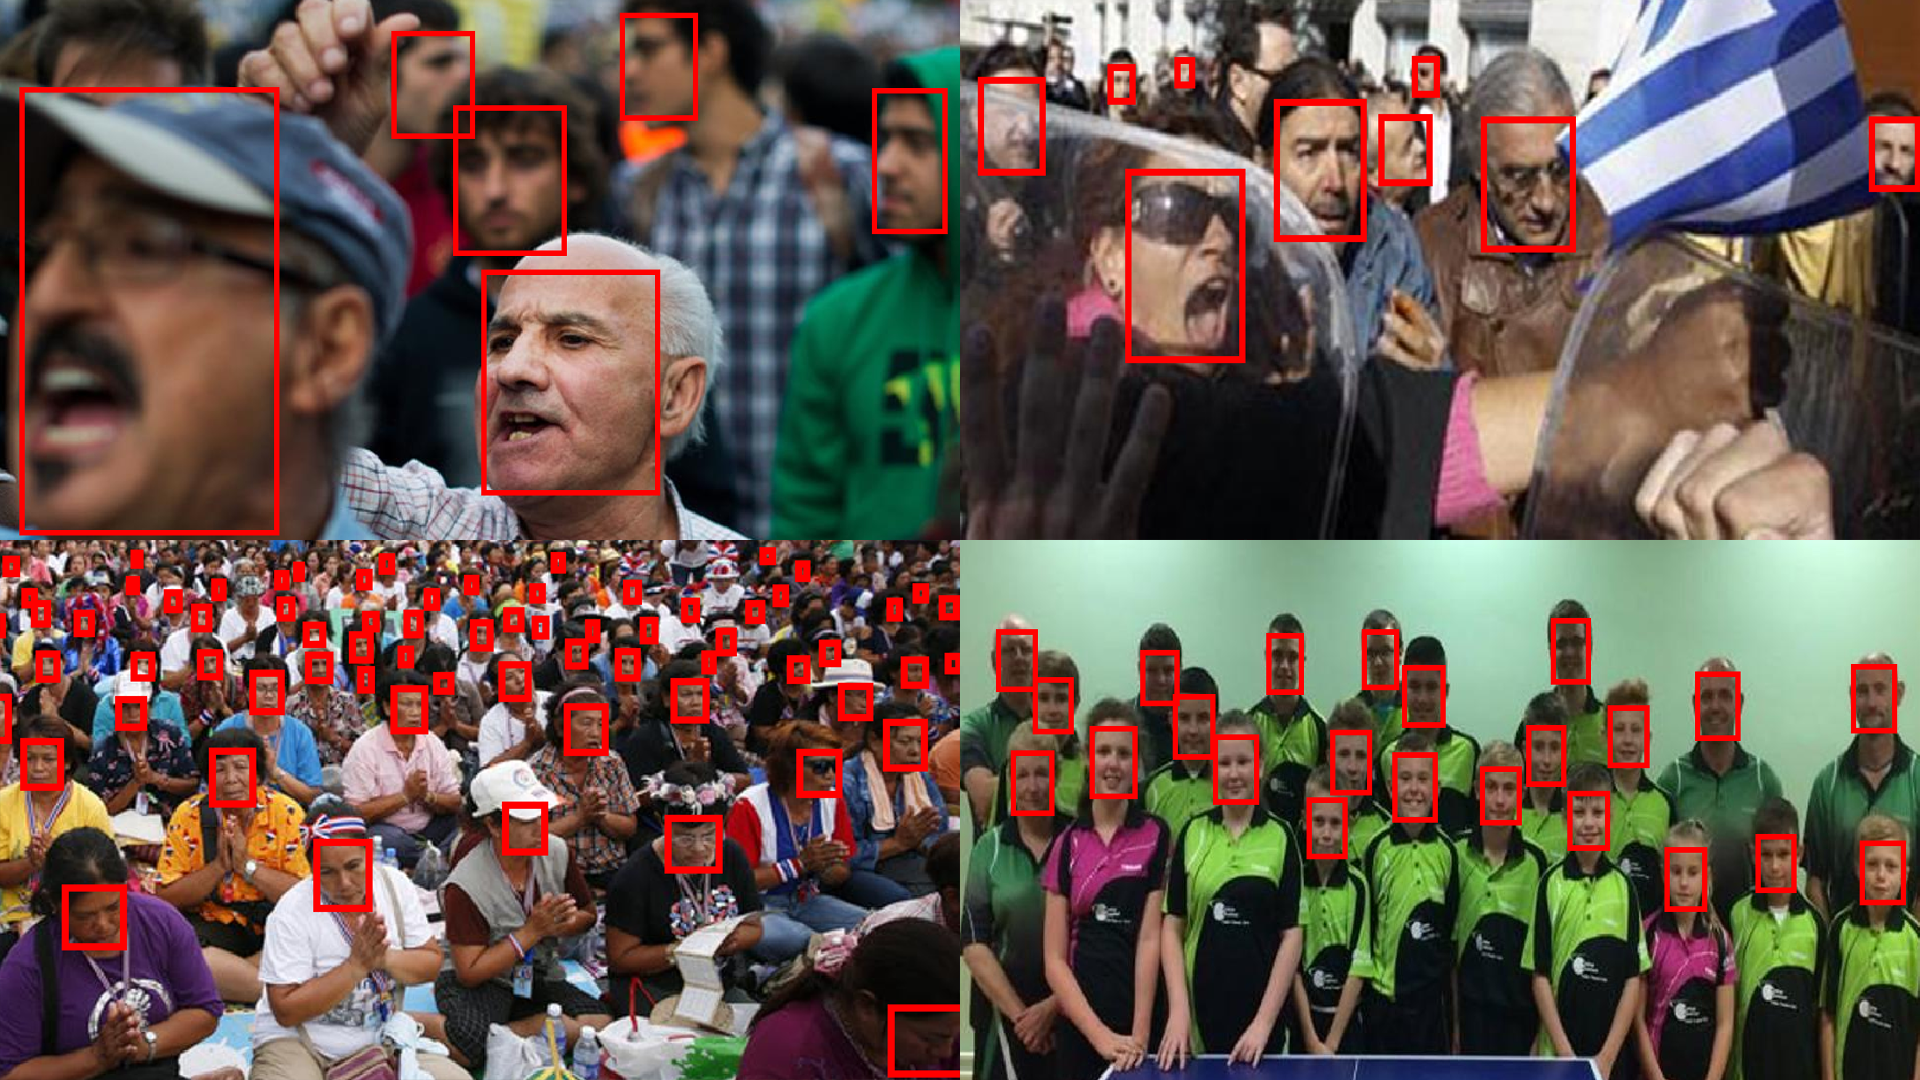
\includegraphics[width=16cm]{figfacedetection.png}\caption{The detections of FaceNet v2.3 on four images of the WIDERFace validation set \cite{WIDERFace}.} \label{figwiderfaceval}
\end{center}
\end{figure}

\subsection{Discussion}
Contrary to research done on multi-class object detection, various methods which have shown to increase accuracy, such as online hard example mining and focal loss, has led to a decrease in accuracy. Using networks of larger depth, as research shows \cite{retinanet} \cite{resnet}, should also increase the accuracy of models, but the contrary was found in this study.

One reason for which the deeper networks, ResNet-50, ResNet-101 and ResNet-151, failed to detect any positive examples, might be the batch size. Since the early experiments used a ResNet-18 as a backbone network, a larger batch size could be used due to smaller model size. This larger batch size could reduce the stochasticity of the SGD by giving a more accuracy approximation of the true gradient. Using a small batch size could have led the model to converge to only detect negative bounding box suggestions.


\section{Improving temporal convolutional networks}
\subsection{Background}
In conventional convolutional neural networks, the model learns to transform a given input by learning to apply a number of two-dimensional discrete convolutions on the input data. Instead of convolving along the spatial dimensions, a convolutional neural network can be used to convolve along the time dimension, and can thus be used as a sequence model for time series data, as long as there is no information leakage from the future into the past. Recent work on Temporal Convolutional Networks (TCN) \cite{tcn} shows that the convolutional model outperforms its recurrant neural network (RNN) variants, including Long Short Term Memory (LSTM), and Gated Recurrent Units (GRU). 

\subsection{Method}
Given a number of data points at timesteps $t = 1, 2, 3, ..., m$, a sequence model sets out to predict the value at timestep $t = m+1$, through the use of information from the earlier timesteps. A temporal convolutional neural network can achieve this by learning to apply a number of 1-dimensional discrete convolutions across all the available previous timesteps, through the use of smart zero-padding to avoid information leakage from the future into the past.

The activations at layer $l$ is a tensor of order 3 $X^{(l)} \in \mathbb{R}^{R \times C \times T}$ where $C$ is the number of feature channels and $T$ is the maximum length of the sequence. The convolutional weights are also a tensor of order 3 $W^l \in \mathbb{R}^{C' \times C \times k}$, where $C'$ is the number of feature channels of the proceeding layer, and $k$ is the kernel size. In addition to the kernel size $k$ and stride $s$, temporal convolutional layers have one additional hyperparameter compared to conventional convolutions, namely a dilation factor $d$. The dilation controls how the kernel is applied on the activations by allowing the kernel to be spaced out across the activation of neurons (see figure \ref{figTCNdil}). The dilated convolution is expressed as:

\begin{equation}
\begin{split}
	X^{(l+1)}_{r, c', t'}	
		& = \sum^{C}_{c=1} \sum^{k}_{i=1} X^{(l)}_{r, c, (1 + st'-s+di)}W^{(l)}_{c', c, i}
\end{split}
\end{equation}

\begin{figure}[h]
\begin{center}
    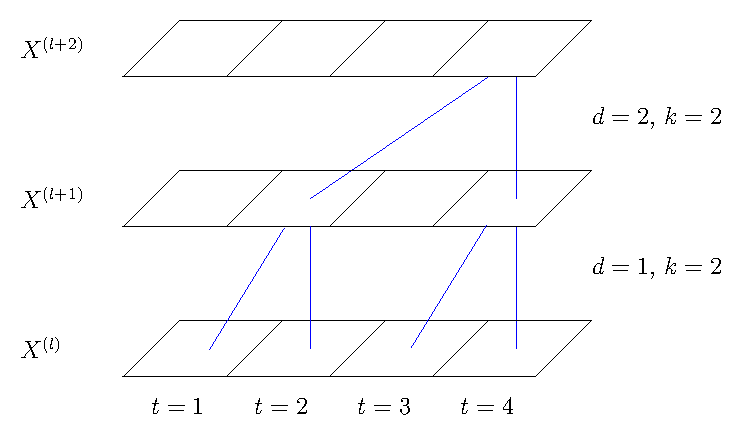
\includegraphics[width=9cm]{figTCNdil.eps}\caption{An illustration of a temporal convolutional network. Every square represents the activations at a single timestep. The different layers of activations represent the layers in the temporal convolutional network. Blue lines represent the kernel applied at a single position on the activation tensor.} 
    
    \label{figTCNdil}
\end{center}
\end{figure}

While TCNs \cite{tcn} were shown to beat the current state of the art in two tasks, SequenceMNIST and the more difficult version PMNIST, I want to adress and improve two problem areas I see with the author's implementation of temporal convolutional networks, namely their zero-padding and dilation scheme.

\subsubsection{Smart zero-padding}
The temporal dimension size $T$ and $T'$ of layers $l$ and $l+1$ respectively can vary in size since they can be convolved upon by a kernel with kernel size $k \geq 1$. More specifically, $T'$ is dependent on $T$ and five hyperparameters: The zero-padding $p_{left}$ and $p_{right}$, the stride $s$, the kernel size $k$, and the dilation $d$.

\begin{equation}
T' = \frac{T-d(k-1)+p_{left}+p_{right}-1}{s}+1
\end{equation}

To not cause any information leakage from a previous timestep at layer $l$ into a future timestep at layer $t+1$, the activation tensor at layer $l$ has to be zero-padded such that $T' \geq T$. The original authors \cite{tcn} solve this problem by padding both sides of the tensor with $p_{left} = p_{right} = d(k-1)$ (when $s=1$). By their method they compute $d(k-1)$ redundant activations which are not used, and which break the rule of information flow from the future into the past, and thus they remove those elements from the tensor before feeding the activations into the next layer. This is a waste of computational resources and can be done in a more efficient way.

I propose only zero-padding the beginning of the activation tensor with zero-padding $p_{left} = d(k-1)$ and $p_{right} = 0$. The result of this is that the activation at timestep $t=k$ can effectively use information from all timesteps $t<k$. At early timesteps, for instance $t=1$, the network is effectively forced to compute convolutions with kernel size 1 since every other neuron which the kernel is on top has a value of 0 due to the zero-padding (see figure \ref{figTCNZeropad}). At later timesteps, the network can make use of the whole kernel, and thus activations and information from earlier timesteps, since it convolves over neurons which were not created by the zero-padding. At the last timestep the network can in theory base its prediction on the whole sequence. The computed activations with my proposed method should be mathematically equivalent to the original authors implementation, but slightly more computationally efficient.


\begin{figure}[h]
\begin{center}
    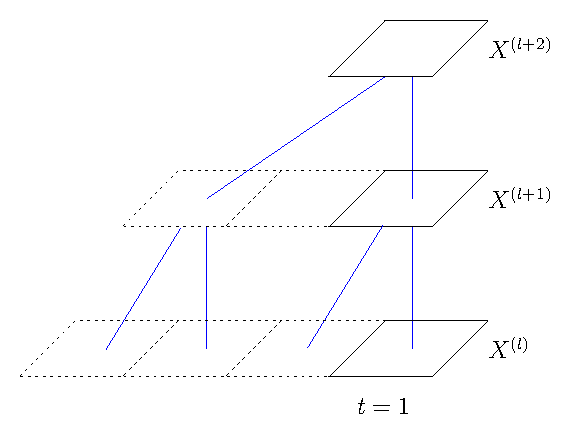
\includegraphics[width=8cm]{figTCNZeropad.eps}\caption{A temporal convolution at timestep $t=1$. Dotted squares represent zero-padded activations, while bold squares represent normal activations. Blue lines represent the convolutional kernel. The network is effectively computing convolutions with kernel size $k=1$ since every neuron except at the first timestep is a neuron created by the zero-padding.}\label{figTCNZeropad}
\end{center}
\end{figure}

\subsubsection{Linear versus exponential dilation increase}
The original authors propose increasing the dilation by a factor of two at every layer. The dilations enable the output neurons to have a bigger receptive field. The receptive field of an output neuron is the maximum amount of input neurons the model can base its prediction of. The receptive field $r$ at layer $l$ for a neuron with kernel size $k$ and dilation $d$ at layer $l-1$ is defined by: 
\begin{equation}
r(d, k) = d(k-1) +1
\end{equation}
Let $L$ be the amount of layers in the temporal convolutional network. The total receptive field $R_{output}$ of an output neuron at layer $L$ on the input layer is given by:
\begin{equation}
R_{output} = 1+\sum^L_{l=2} (r(d_l, k_l) -1)
\end{equation}
Here $d_l$ and $k_l$ is the receptive field and kernel size of the single neuron in layer $l$, on the previous layer $l-1$.

I suggest increasing the dilation of the layers linearly instead of exponentially. Firstly, a too big of an increase of dilation causes the last layers with kernel size $k \leq 2$ to effectively turn into convolutions with kernel size $k=1$. This is due to that every kernel weight, except those at the same timestep, is being multiplied by a zero-padded neuron. The rest of the kernel will be placed on intervals of $d$ timesteps earlier. If $d$ is large enough, the next activation used in the convolution will always be a zero-padded neuron, and thus the whole layer effectively becomes a convolution with kernel size $k=1$, similar to what's illustrated in figure \ref{figTCNZeropad}. The effect of exponential dilations in deep architectures is that only the first layers use data from previous timesteps, while later layers simply become mathematically equivalent to normal feed-foward layers across a single timestep.

Secondly, because a temporal convolutional network has to preserve its temporal dimension $T$ at every layer through the use of zero-padding, an exponentially increasing dilation can cause too much memory usage, since zero-padding increases the memory usage of the model. This is especially important for \cite{tcn} implementation which uses twice as much zero-padding as my implementation.

\subsection{Results}
To show the effects of these changes I compare my implementation with the suggested modifications to the model, with the original TCN model \cite{tcn} on two different tasks.

\subsubsection{SequenceMNIST (SeqMNIST)}
SequenceMNIST is a task which uses the MNIST database of handwritten digits \cite{MNIST}. A model is sequentially given the pixels in the image, one by one, as a sequence of size $784$, and is then asked to predict what digit the image was of. The problem was formulated to evaluate sequence models ability to withhold memory across large timesteps.

\subsubsection{Permuted SequenceMNIST (PMNIST)}
Permuted SequenceMNIST (PMNIST) is a more difficult deviation of the SequenceMNIST task where every pixel in the image is randomly permuted. All images are randomly permuted the same way, and the model is evaluated on images permuted similar to the training data.

\subsubsection{Experiments}
Three different model architectures were tested on SeqMNIST and PMNIST, namely three models with different residual blocks: Single, Double, and Radical. The Single residual block is the block used in the original TCN \cite{tcn} architecture. It uses two layers made up of a sequence of a convolution, weight normalization of the kernel weights, ReLU activation and dropout. Weight normalization normalizes the kernel weights such that its direction remains constant, while changing the magnitude of the tensor \cite{pytorch}. Dropout randomly sets an activation to be equal to zero during training \cite{cs231n}. The input to the sequential layers is then added element-wise to its output to create the final activations of the last layer. This is called a residual connection. The residual connection in the Simple block is between every second convolution. The Double residual block has an addition residual connections which connects the activations of the first convolution in block $b$ to the activations of the first convolutional block in layer $b+1$. The Radical residual block has 4 convolutions and uses residual connections between the input and the output, the input and the second convolution, the second convolution and the output, and the first convolution and the third convolution. The three architectures are illustrated in figure \ref{figTCNGraph}. The Radical block is additionally illustrated in figure \ref{figTCNRadical}.

\begin{figure}%[h]
\begin{center}
    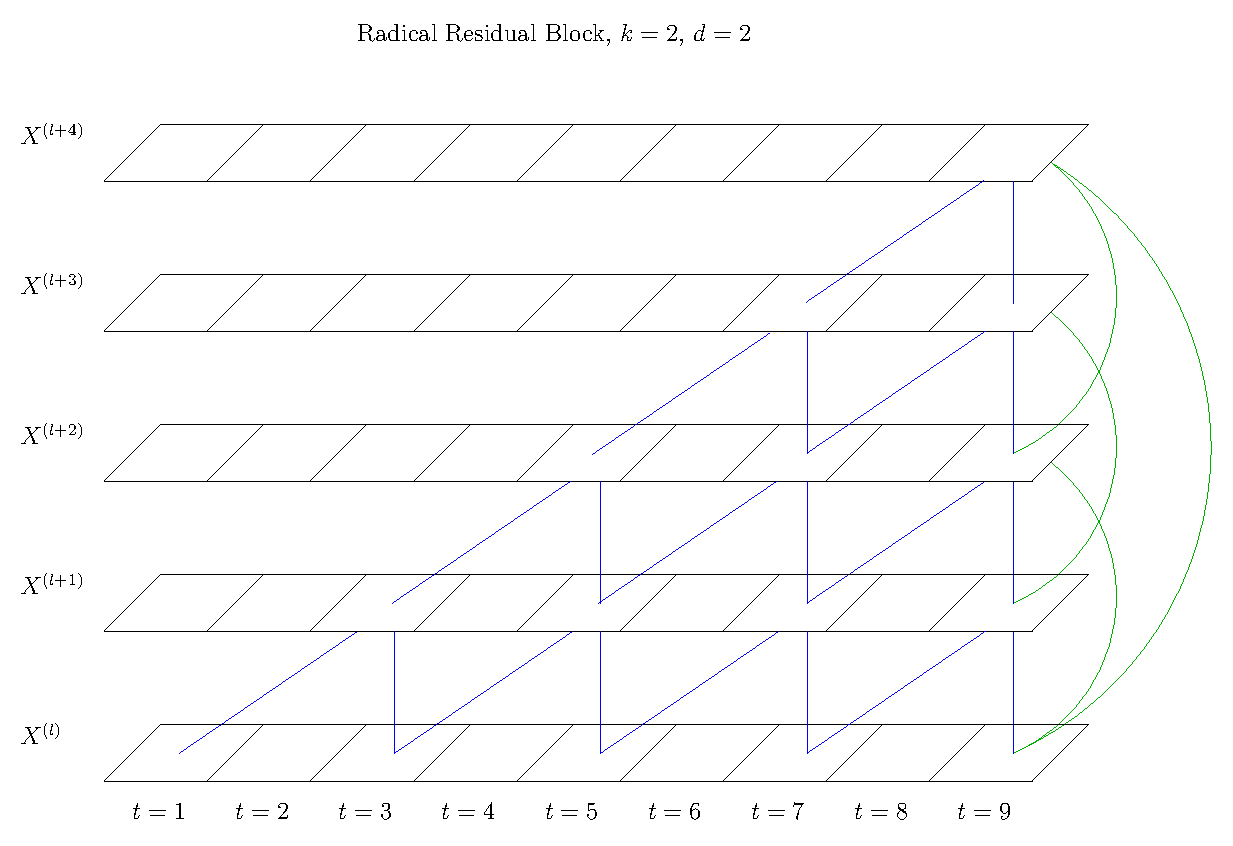
\includegraphics[width=10cm]{figRadical.eps}\caption{An illustration of a temporal convolutional network. Every square represents the activations at a single timestep. Blue lines represent the kernel applied at a single temporal position on the activation tensor. Green lines represent residual connections between two convolutional layers.}\label{figTCNRadical}
\end{center}
\end{figure}

\begin{figure}%[h]
\begin{center}
    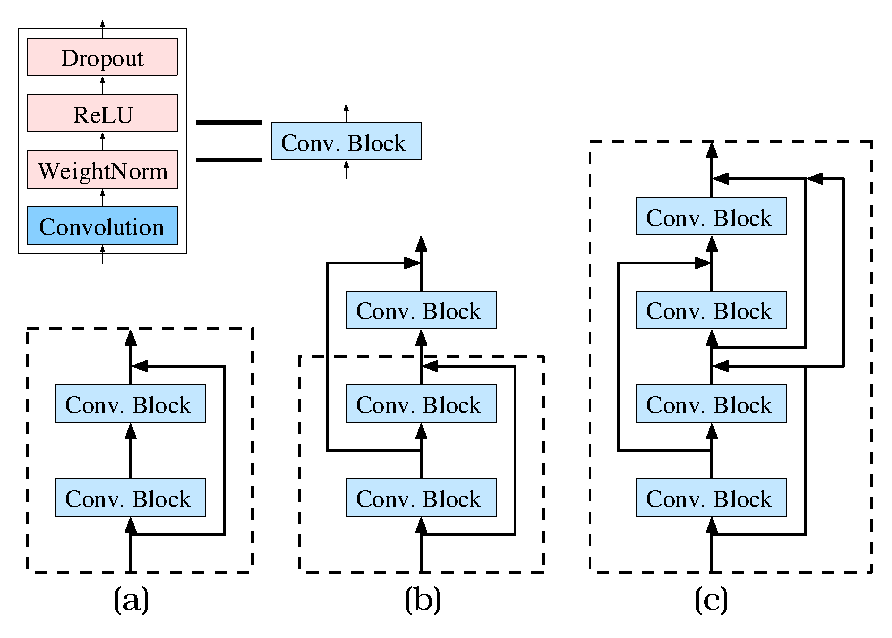
\includegraphics[width=16cm]{figGraph.eps}\caption{The proposed (a) Single, (b) Double and (c) Radical residual blocks. Every convolution is proceeded by ReLU activations and dropout, and uses weight normalization. The Single block has a residual connection every 2 convolutional layers. The Double block has an addition residual connections which connects the activations of the first convolution in block $l$ to the activations of the first convolutional block in layer $l+1$. The Radical residual block has 4 convolutions and uses residual connections between the input and output, input and the second convolution, the second convolution and the output, and the first convolution and the third convolution.}\label{figTCNGraph}
\end{center}
\end{figure}

The network hyperparameters were picked on the basis of the output neurons having a receptive field bigger than, but not much greater than, the maximum sequence size of 784 timesteps, while being as close as possible to the original TCN model \cite{tcn}. The Single and Double model uses 12 Single blocks, with dilations $d_b=3b-2$ at block $b$. The Radical model uses 6 Radical blocks, with dilations $d_b=6b-5$ at block $b$. The kernel sizes were picked to be the same as the original TCN, namely $k=6$. The total receptive field is 1001 timesteps for the Single and Double model, and 1021 timesteps for the radical model. Every model uses a total of 24 convolutions. The channel size was set to 32, except for the output layer which has 10 channels, one for every digit. The final prediction tensor is put into a softmax function to transform the output into interpretable probabilities. At every timestep $t$ the model predict $R \times 10$ probabilities that the image is of a specific digit. Here $R$ is the batch size. Following \cite{tcn}, the model is only evaluated and trained on the prediction of the last timestep.

5 000 samples in the training set were randomly picked to create a validation set to track during training. The remaining 55 000 images were used to create the new training set. All models were trained simultaneously on the same randomly picked mini-batches of 100 images.

During early experiments, the Double and Radical models diverged when using a too high learning rate. To combat the models started with a learning rate of 0.001, which was, during later iterations, increased by a factor of 10.

For SeqMNIST, the models were trained for 100 000 iterations using SGD with momentum. The learning rate was increased by a factor of 10 after 200 and 1000 iterations, and decreased by a factor of 10 after 70 000 and 90 000 iterations.

For PMNIST, the models were trained for 200 000 iterations using SGD with momentum. The learning rate was increased by a factor of 10 after 200 and 1000 iterations, and decreased by a factor of 10 after 130 000 and 180 000 iterations.

Figures \ref{figseqmnistloss} to \ref{figpmnistacc} show the loss functions of the training and validation sets, and the validation accuracies of all three models, on the SeqMNIST and PMNIST tasks.

\begin{figure}
\begin{center}
    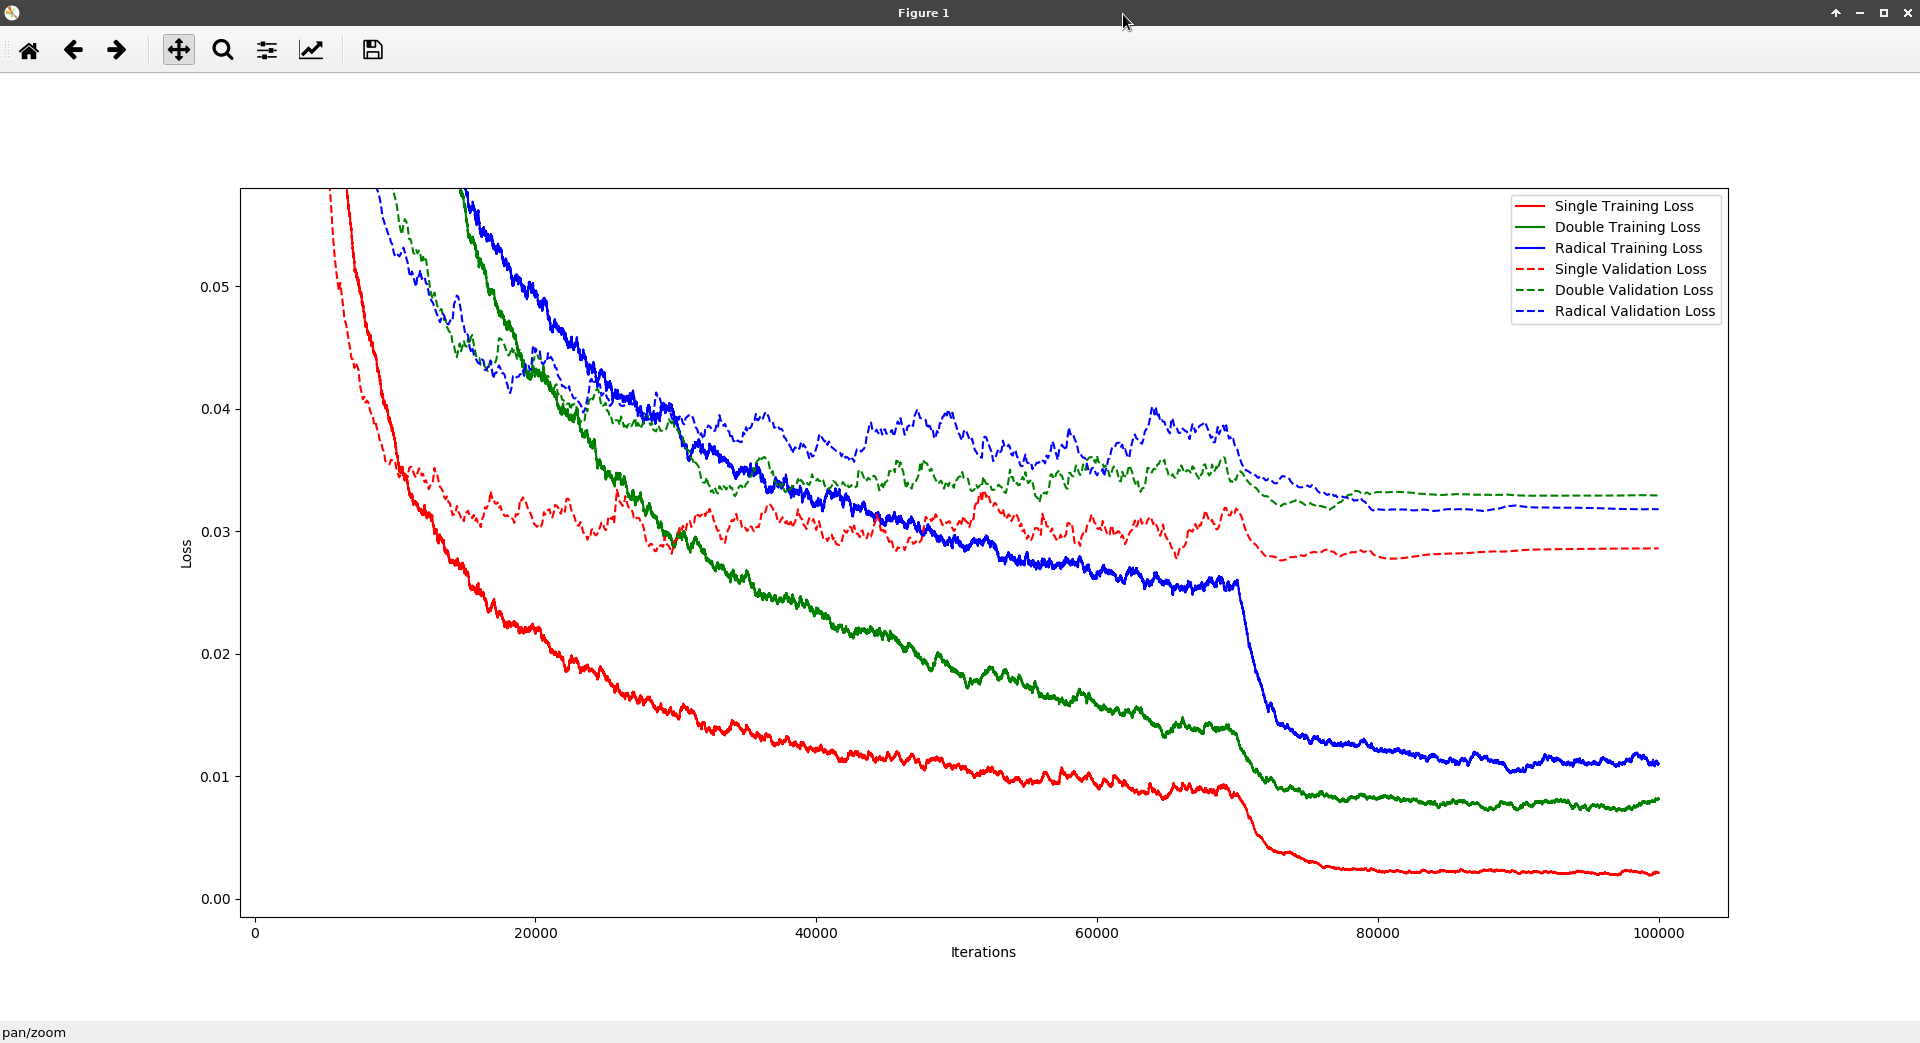
\includegraphics[width=15cm]{seqmnistloss.png}\caption{The training loss on SequenceMNIST of the three models with the Single, Double, and Radical residual blocks. Bold lines show the loss on the training set while dotted lines show the loss on the validation set.}\label{figseqmnistloss}
\end{center}
\end{figure}
\begin{figure}
\begin{center}
    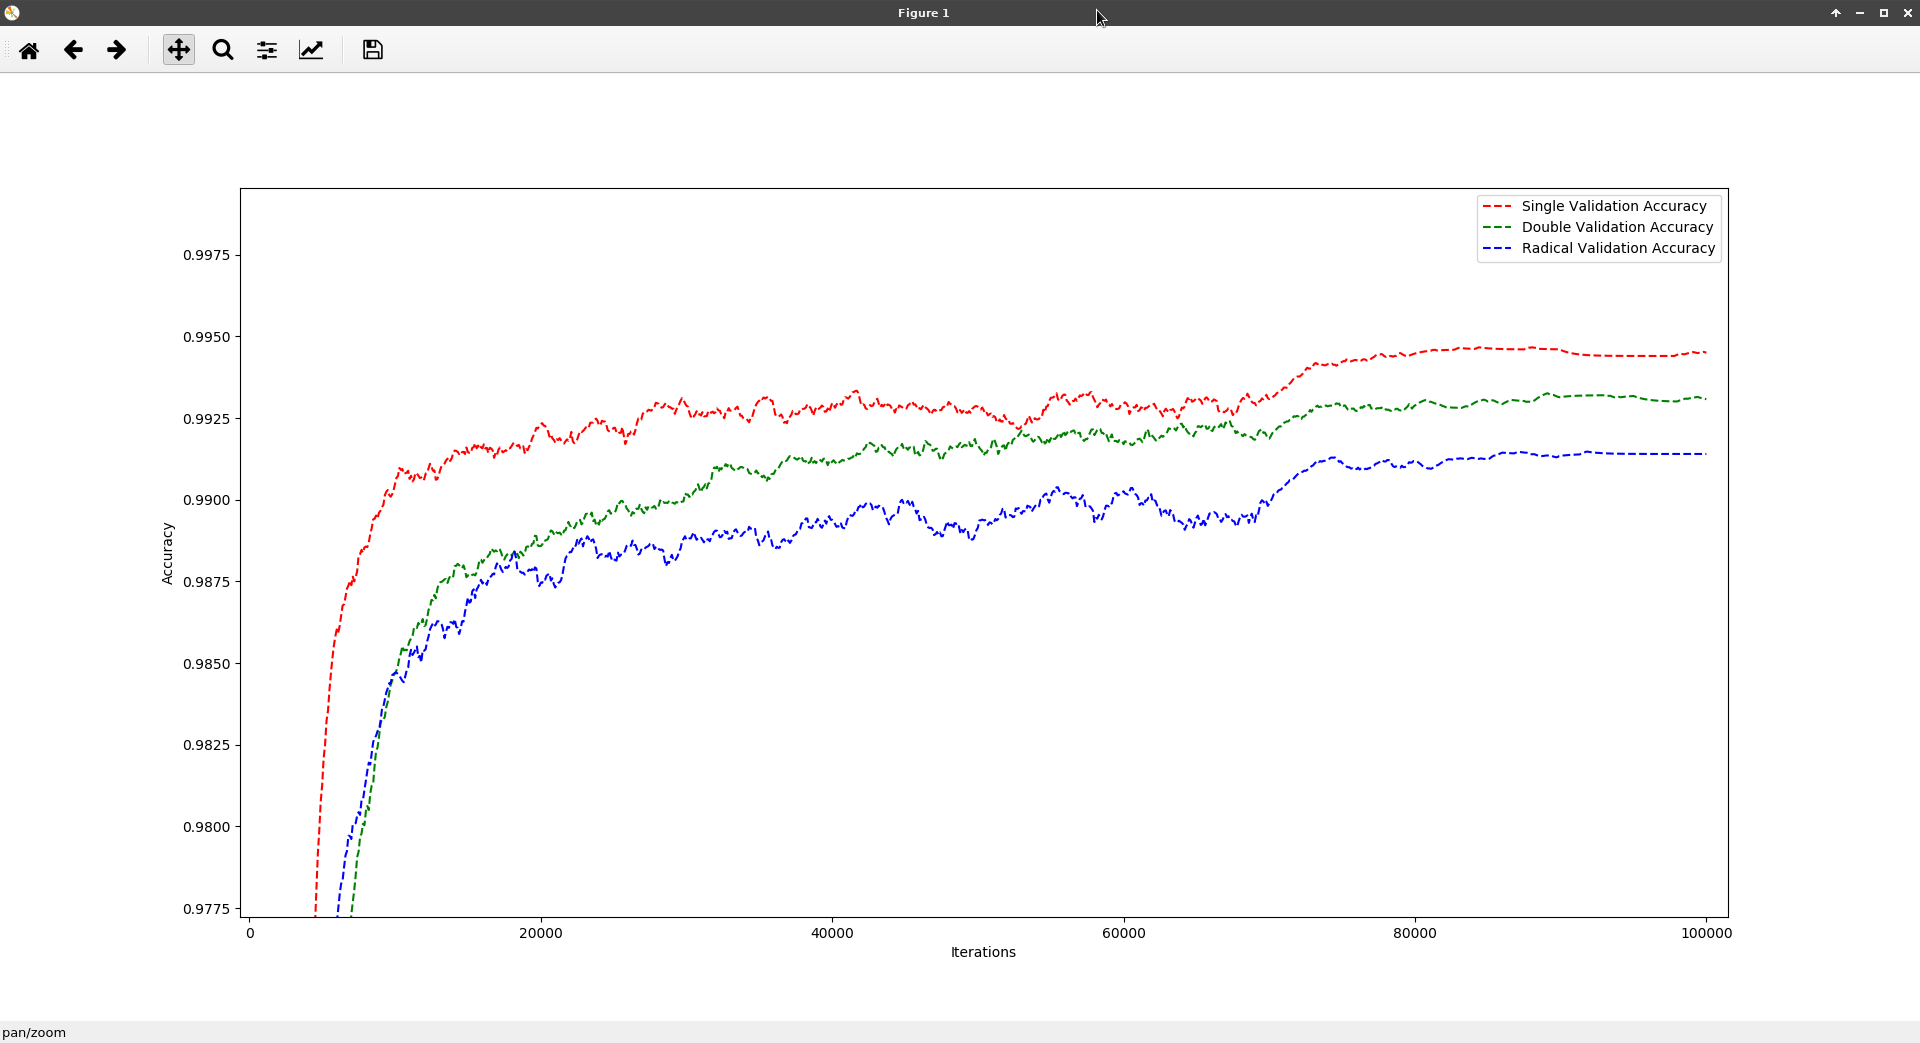
\includegraphics[width=15cm]{seqmnistacc.png}\caption{The validation accuracy on SequenceMNIST of the three models with the Single, Double, and Radical residual blocks. The accuracy is measured as the percentage of correctly classified images over the whole validation set.}\label{figseqmnistacc}
\end{center}
\end{figure}
\begin{figure}
\begin{center}
    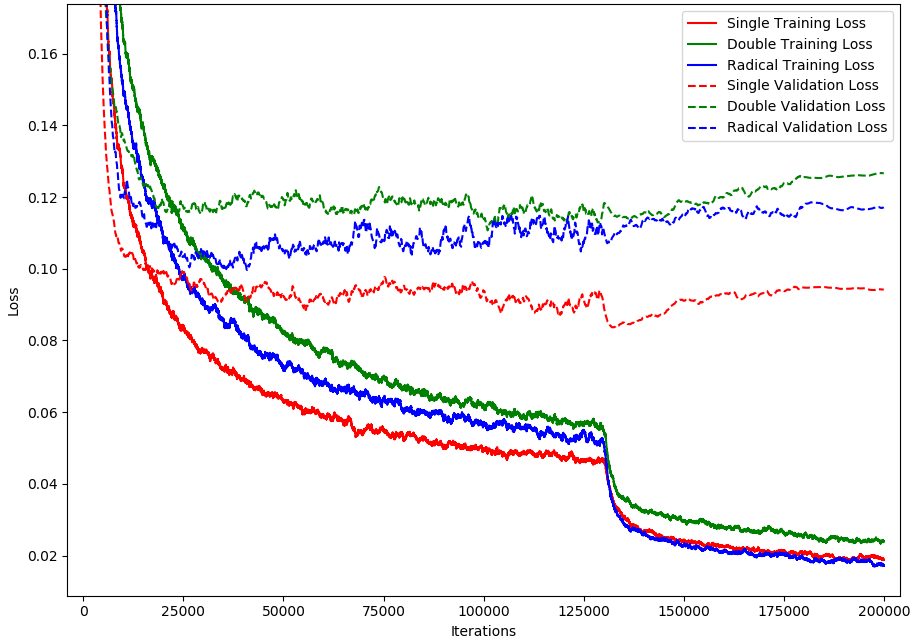
\includegraphics[width=15cm]{pmnistloss.png}\caption{The training loss on PMNIST of the three models with the Single, Double, and Radical residual blocks. Bold lines show the loss on the training set while dotted lines show the loss on the validation set.}\label{figpmnistloss}
\end{center}
\end{figure}
\begin{figure}
\begin{center}
    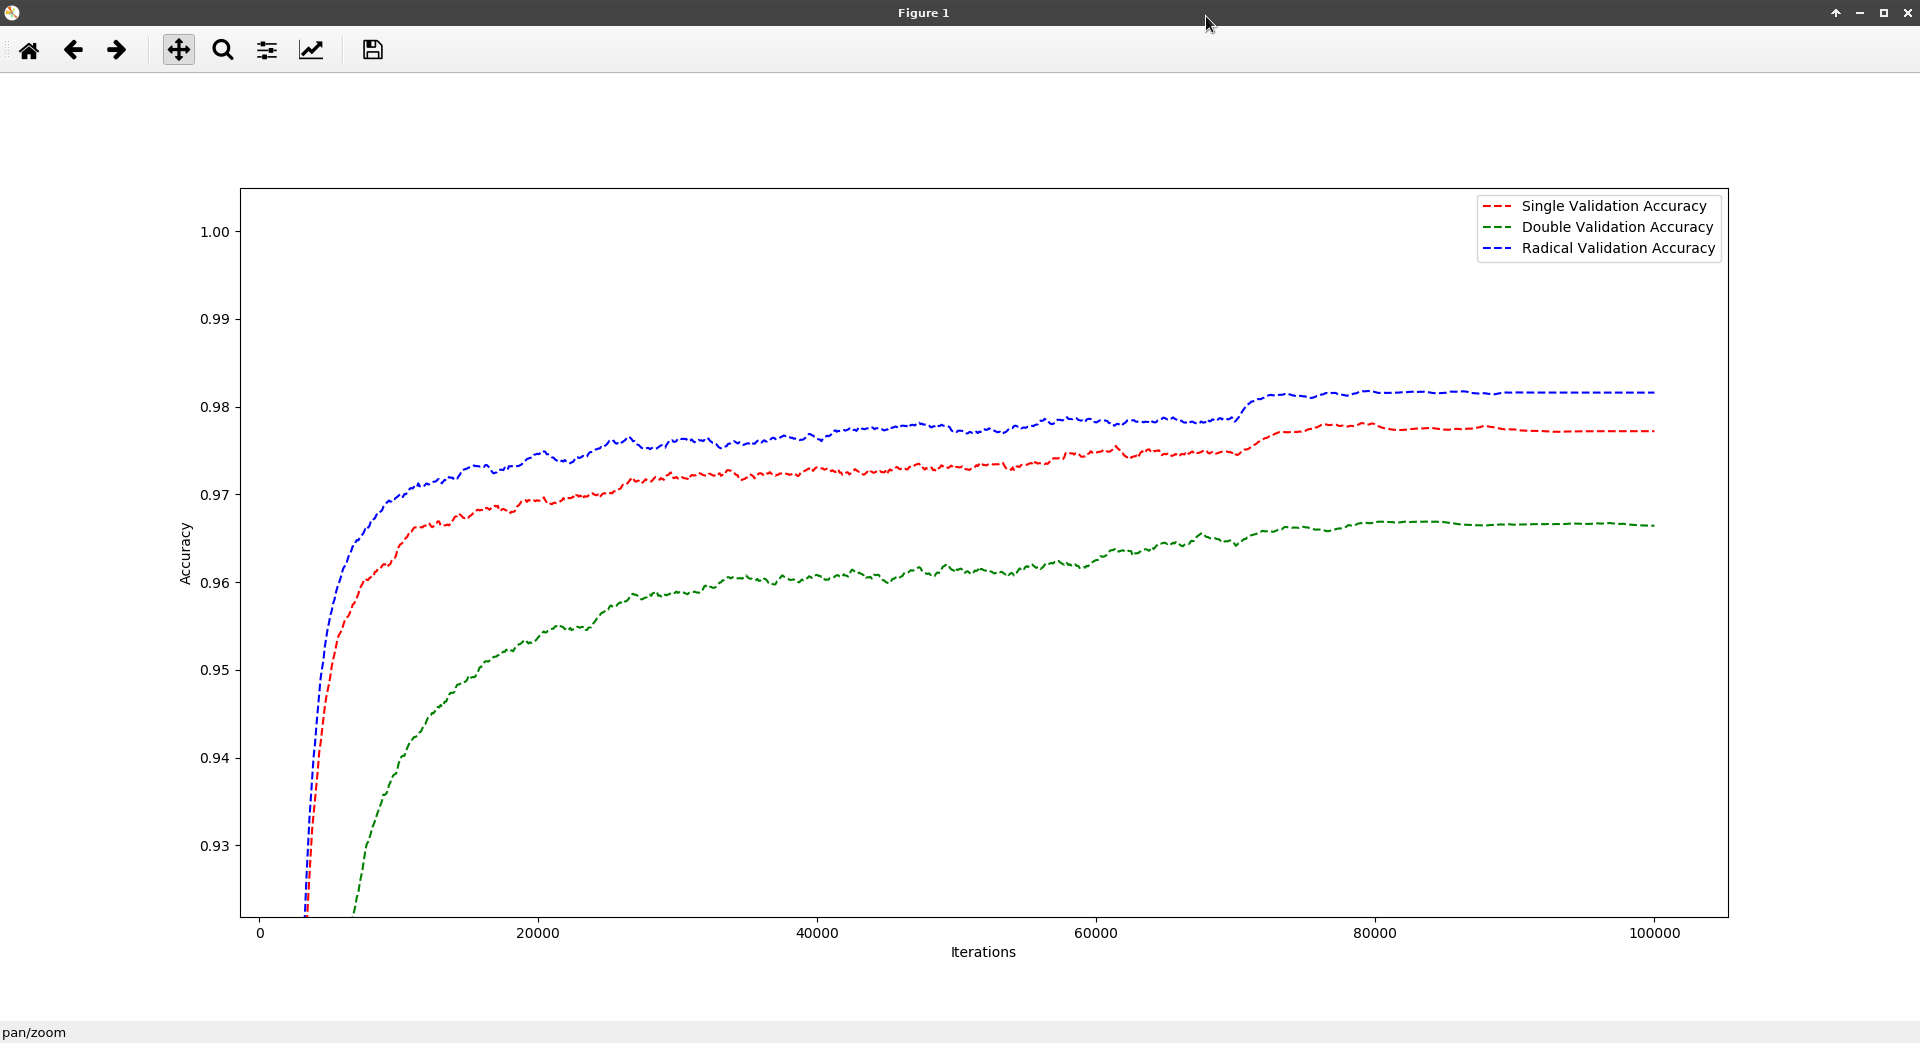
\includegraphics[width=15cm]{pmnistacc.png}\caption{The validation accuracy on PMNIST of the three models with the Single, Double, and Radical residual blocks. The accuracy is measured as the percentage of correctly classified images over the whole validation set.}\label{figpmnistacc}
\end{center}
\end{figure}

When evaluated on the test set, all models beat the current state of the art on both tasks. The Single model performed best on the test set, but was beaten by the Radical model on the SeqMNIST task regarding validation accuracy and loss.

\begin{table}
\begin{center}
    \begin{tabular}{| l | l | l | l | l | l |}
    \hline
    Model & Test Acc. & Val. Acc. & Val. Loss & Train Loss\\ \hline \hline
    TCN (Single) & \textbf{99.53\%} & 99.23\% & 0.046 & \textbf{0.006} \\ \hline
    TCN (Double) & 99.34\% & 99.07\% & 0.050 & 0.014 \\ \hline
    TCN (Radical) & 99.37\% & \textbf{99.30\%} & \textbf{0.040} & 0.010 \\ \hline
    Dilated GRU \cite{dilatedgru} & 99.0\% & N/A & N/A & N/A \\ \hline
    TCN (Original) \cite{tcn} & 99.0\% & N/A & N/A & N/A \\ \hline
    \end{tabular}
    \caption{\textbf{SequenceMNIST}. A table comparing my proposed modified temporal convolutional networks with the current state of the art on the SequenceMNIST task.} \label{tabseqmnist}
\end{center}
\end{table}

\begin{table}
\begin{center}
    \begin{tabular}{| l | l | l | l | l | l |}
    \hline
    Model & Test Acc. & Val. Acc. & Val. Loss & Train Loss\\ \hline \hline
    TCN (Single) & \textbf{97.86\%} & \textbf{98.28\%} & \textbf{0.094}  & 0.019 \\ \hline
    TCN (Double) & 97.36\% & 98.10\% & 0.126  & 0.024 \\ \hline
    TCN (Radical) & 97.82\% & 97.94\% & 0.117  & \textbf{0.017} \\ \hline
    TCN (Original) \cite{tcn} & 97.2\% & N/A & N/A & N/A \\ \hline
    \end{tabular}
    \caption{\textbf{Permuted SequenceMNIST}. A table comparing my proposed modified temporal convolutional networks with the current state of the art on the Permuted SequenceMNIST task.} \label{tabpmnist}
\end{center}
\end{table}

\subsection{Discussion}
The changes are shown to increase the accuracy of the temporal convolutional model, across all three residual building blocks and both tasks, beating the previous state of the art.  The error rate for Sequential MNIST is halved, compared the the old model, using the new methods.

\section{Evaluation of TCNs for image captioning}
\subsection{MSCOCO caption dataset}
The MSCOCO caption dataset \cite{mscoco} is a dataset containing 164 062 images and a total of 1 026 459 human labeled image captions. This paper uses the 2017 train/val split of 115 000 images in the training set, and 5 000 images in the validation set. The remaining images are contained in the test set with the ground truth not publicly available.

\subsection{Background}
In the Stanford course \textit{Convolutional Neural Networks for Computer Vision} \cite{cs231n}, the lecturer demonstrated that a deep convolutional neural network could be used as a feature extractor in conjunction with a recurrent neural network (RNN) to sequentially generate an image caption. In this following section. A closer look on the current state of the art on image captioning, at the MSCOCO caption leaderboards, reveals that recurrent neural-network-based architectures are used, mainly LSTMs and GRUs. Therefore it is of interest to apply the newly high performing sequence model, temporal convolutional networks (TCN) \cite{tcn}, to the area of automatic image captioning, to compare its performance with the current recurrent architectures. Two models will be trained and compared head-to-head on the task of automatic image captioning: The temporal convolutional network model and the gated recurrent unit model.

\subsection{Sequential sentence modeling}
The models generate image captions by sequentially suggesting the next word in a sentence, from a large vocabulary of allowed words to choose from. The vocabulary was chosen to be limited to every word in the training captions which appear five our more times. Only captions in the training set were used, ignoring the available captions in the validation set, to make the results on the validation more closely resemble the results which will be gotten on the test set. Capitalization and special characters were ignored when generating the vocabulary. The final vocabulary size was approximately 10 000 words. Words in the training image captions not included in the vocabulary were replaced with an unknown token: \textit{<UKN>}. The vocabulary also includes an end of string token, \textit{<EOS>}, used by the models to signal that the generated sentence is complete.

Each word is represented as a one-hot vector encoding, where every element but one is set to zero, and the index of the non-zero element determines what word it is. Vector embeddings into continuous space (PyTorch's nn.Embeddings) \cite{pytorch} are used map the one-hot representations into a vector of a specific dimension.

During training, each word is given sequentially to the model, and the model is asked to predict the next word in the sentence. It does this by predicting a vector with $N$ values, where $N$ is the vocabulary size. The vector is then put into a softmax function, and its elements are interpreted as the probability that the selected word should be the next word in the sentence. The model does not ignore the \textit{<UKN>} tokens, and trains to predict them the same as any other word. At test time if \textit{<UKN>} were to be picked, it is replaced by the word prediction with the second highest probability.

\subsection{Loss function}
The loss function $L(\theta)$ used for automatic image captioning is cross entropy \cite{notesonbackprop}. Let $M$ be the combined number of words of all the captions in the mini-batch, and $S$ be the set of all predicted word probabilities $p$. $\hat{p}$ is the associated ground truth to word prediction $p$. The total loss if given by:

\begin{equation}
L(\theta) = \frac{1}{M} \sum_{p \in S} p \log{\hat{p}}
\end{equation}

\subsection{TCN}
Based on the results of the previous section regarding improvements on temporal convolutional networks, a model without an exponentially increasing dilation will be used. One additional reason for this is because the sequence size is small, approximately never larger than 30 timesteps (30 words per sentence). Using an exponentially increasing dilation $d_l = 2^{l-1}$ at layer $l$ would result in the network becoming a series of convolutions with kernel size $k=1$ (mathematically equivalent to a fully connected/feed-forward layer) at layers $l>5$. To avoid this, the dilations were picked to make the output neurons receptive field to be equal to approximately 40 timesteps. For simplicity, and because the performance difference of the Single, Double and Radical residual blocks were only marginal, the most basic block is picked: The Single residual block (see figure \ref{figTCNGraph}). 
Following \cite{tcn} advancements with TCNs on sentence modeling tasks, a kernel size $k=2$ was used. A total of $18$ residual blocks were used. The dilations were subsequently picked to be $d=1$ for every convolution, for a total receptive field of $39$ timesteps.

The word embeddings use 512 channels, and every convolution uses 256 channels, except the last layer which uses $N \approx $ 10 000 channels, where $N$ is the vocabulary size. A given image is fed into a ResNet-18, up to and including the global average pooling layer, as a feature extractor to extract a 512-feature vector from the image. This feature vector is used as a start of string token and is given to the TCN as a "word" at the first timestep.

At runtime, the model only has access to the 512-dimensional feature vector from the image. The model predicts the next words in the sentence sequentially from the previous available words. At timestep $t=1$, only the feature vector from the ResNet-18 is used. At the next timesteps, the embedded predicted word from the previous timestep is concatenated to the end of the activation tensor at the first layer. To predict the next word in the sequence, the model performs convolutions on the concatenated tensor. This process is repeated until the model predicts an end of string \textit{<EOS>} token.

\subsection{GRU}
The second model tested is a model often used for image captioning and sequential data, a derivation of a normal recurrent neural network \cite{cs231n} CITE CITE mscoco leaderboards]. The architecture used follows industry standards for GRUs. A ResNet-18 is used, the same as for the TCN model, to predict a 512-dimensional feature vector from the image. This vector is set as the first hidden layer in the GRU. The feature vector is additionally used as a start of string token, similar to the TCN model. Three hidden layers of size 512 are used. The vocabulary used by the GRU is the same as the one used by the TCN. Word embeddings of size 512 are used, similar to the TCN model, to represent words as tensors.

At runtime, keeping all the previous words in memory is not required, unlike the TCN model. To generate an image caption, the ResNet-18 feature vector is given to the GRU as a start of string token. The predicted word is then embedded and given to the model, to predict the next word in the sentence. This process is repeated until the model predicts an end of string \textit{<EOS>} token.

\subsection{Results}
Early experiments used the more commonly used ResNet-50 as a feature extractor, but the TCN model would not fit into 11GB of VRAM GPU memory during training, and could thus not be used. The GRU did not have any memory problems. Further experimentation reverted to the less deep ResNet-18 for both models.

Each model was trained for 1.75 million iterations on the training set of the MSCOCO dataset, using the train/val 115k/5k split. The validation loss was tracked during training, but was not used by SGD. The models were trained on images resized to $224 \times 224$ pixels, with a batch size of 2 due to memory limitations, the absolute minimum for batch normalization to function. Each image used 5 randomly chosen ground truth image captions during training. An initial learning rate of 0.1 was used for both models, which was divided by a factor of 10 after 1 million iterations, and 1.5 million iterations. Table \ref{tabimagecaptioning} shows the final result on the 5 evaluation metrics used by the MSCOCO test set evaluation server: CIDEr-D, METEOR, Rogue-L, BLUE and SPICE. Figure \ref{figimagecaptioning} shows quantitative results on the MSCOCO Captions validation set.

\begin{table}
\begin{center}
    \begin{tabular}{| l | l | l | l | l | l| l | l  |}
    \hline
    Model & CIDEr-D & METEOR & Rouge-L & BLUE-1 & BLUE-2 & BLUE-3 & BLUE-4\\ \hline \hline
    TCN (C40) & 0.729 & 0.294 & 0.613 & 0.829 & 0.709 & 0.583 & 0.468 \\ \hline
   	GRU (C40) & \textbf{0.752} & \textbf{0.297}& \textbf{0.622}& \textbf{0.841}& \textbf{0.727}& \textbf{0.600}& \textbf{0.483}\\ \hline \hline
    TCN (C5) & 0.722 & 0.219& 0.482& 0.658& 0.476& 0.338& 0.240\\ \hline
    GRU (C5) & \textbf{0.741} & \textbf{0.222}& \textbf{0.490}& \textbf{0.668}& \textbf{0.488}& \textbf{0.347}& \textbf{0.248}\\ \hline
    \end{tabular}
    \caption{\textbf{MSCOCO Caption Results}. A table comparing the results of the temporal convolutional model (TCN) to a Gated Recurrent Unit (GRU) on the evaluation metrics used by the MSCOCO Caption evaluation server. Bold scores show the best results.} \label{tabimagecaptioning}
\end{center}
\end{table}

\begin{figure}[h]
\begin{center}
    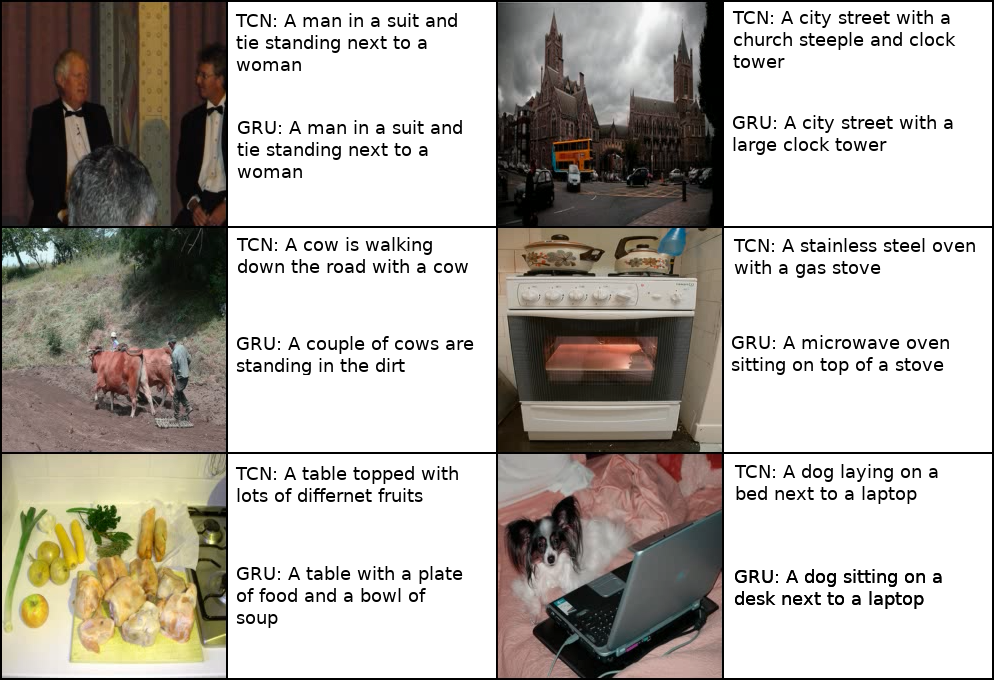
\includegraphics[width=15cm]{captionsbig.png}\caption{Comparative results of the TCN and GRU model on images from the MSCOCO Captions validation set \cite{mscoco}.} \label{figimagecaptioning}
\end{center}
\end{figure}

\subsection{Discussion}
The temporal convolutional network performed marginally worse across all evaluation metrics compared to the recurrent model. While the convolutional model converged faster on the training set, it failed to generalize to the validation set, shown by the tracked loss function in figure \ref{figimagecaptioning}.

One reason might be that the TCN couldn't effectively make use of the features generated by the backbone feature extractor ResNet. The GRU had a very efficient method of storing the image features in its first hidden layer, which can be kept in the models memory during the whole sequence. The TCN only has access to the input image features from a single timestep. Even though the output neurons had a receptive field of 39 timesteps, and thus could make use the image features at every timestep, it is possible that this method of incorporating the image features at every timestep is not sufficient to generate accurate predictions. The TCN might just be predicting the next word in the sentence based exclusively on the previous words, with no input from the extracted image features.

A solution to the problem of efficiently representing the image features in the TCN could be to concatenate the extracted image features to the embedded input words at every timestep. Further experimentation has to be done to reach a decisive conclusion regarding this problem.

On the other hand, as quantitative results as shown in figure \ref{figimagecaptioning}, the TCN suggests more accurate captions compared to the GRU model, when evaluated by humans.

\section{Conclusion} 
A mathematical derivation of the general case of a convolutional neural network with an arbitrary input of a tensor of order 4 was presented, with varying strides and zero-padding, including both forward and backpropagation. 

Furthermore, a dense face detector was systematically constructed and improved by investigating how techniques such as the focal loss, feature pyramid networks, and online hard example mining (OHEM) affected the final accuracy of the model. Contrary to previous research, OHEM and focal loss was shown to decrease the accuracy of the object detector. The final model is efficient and accurate enough to function as a real time face detector for surveillance and face tagging systems.

Additionally, the accuracy of temporal convolutional networks could be increased by using a linear dilation increases, together with more efficient zero-padding, to beat the current state of the art, with all three different residual building blocks. Temporal convolutional networks were also shown to be a contender to its recurrent variant, the Gated Recurrent Unit, on the task of automatic image captioning, performing only marginally worse on automatic evaluation metrics, and has the potential to perform better with additional changes. 

\begin{thebibliography}{99}	
 \bibitem{cs231n} 
	\textit{CS231n: Convolutional Neural Networks for Visual Recognition.}
    F. Li, A. Karpathy and J. Johnson.
	Stanford University, university course, winter 2016.
	
	\bibitem{batchnorm} 
	\textit{Batch normalization: Accelerating deep network training by reducing internal covariate shift.}
    S. Ioffe and C. Szegedy. 
	arXiv preprint arXiv:1502.03167, 2015.

\bibitem{eigen}
\textit{Eigen v3}.
G. Guennebaud and B. Jacob and others. URL http://eigen.tuxfamily.org. 2010

\bibitem{numpy}
\textit{The NumPy Array: A Structure for Efficient Numerical Computation, Computing in Science \& Engineering, 13, 22-30}.
S. van der Walt, S. C. Colbert and G. Varoquaux.  (2011), DOI:10.1109/MCSE.2011.37 

 

\bibitem{tensorflow}
\textit{TensorFlow: Large-scale machine learning on heterogeneous systems},
M. Abadi, A. Agarwal, P. Barham, E. Brevdo,
Z. Chen, C. Citro, G. Corrado, A. Davis,
J. Dean, M. Devin, S. Ghemawat, I. Goodfellow,
A.Harp, G. Irving, M. Isard, R. Jozefowicz, Y. Jia,
L. Kaiser, M. Kudlur, J. Levenberg, D. Mané, M. Schuster,
R. Monga, S. Moore, D. Murray, C. Olah, J. Shlens,
B. Steiner, I. Sutskever, K. Talwar, P. Tucker,
V. Vanhoucke, V. Vasudevan, F. Viégas,
O. Vinyals, P. Warden, M. Wattenberg, M. Wicke,
Y. Yu, and X. Zheng.
URL https://www.tensorflow.org/.
2015.

\bibitem{pytorch}
\textit{Automatic differentiation in PyTorch}.
A. Paszke,   S. Gross, S. Chintala,   G. Chanan,   E. Yang,   Z. DeVito,   Z. Lin,   A. Desmaison,   L. Antiga,  and A. Lerer
2017

\bibitem{hidden12}
	\textit{A simple neural network with Python and Keras}.
	A. Rosebrock.
	PyImageSearch
	URL https://www.pyimagesearch.com/.
	26 September 2016.
	
\bibitem{wikiStanford} 
	\textit{Unsupervised Feature Learning and Deep Learning.}
    Standford University, Department of Computer Science.
    URL http://ufldl.stanford.edu/wiki/.
	Last updated 31 Mars 2013.	
	

	
\bibitem{gradient} 
	\textit{Scientific Computing 2013, Worksheet 6: Optimization: Gradient and steepest descent.}
    University of Tartu, Estonia.
    2013.
    
\bibitem{convmath} 
	\textit{Introduction to Convolutional Neural Networks.}
    J. Wu. 
    National Key Lab for Novel Software Technology, Nanjing University, China.
    1 May, 2017.
    
\bibitem{figSGD}
	\textit{Tuning the learning rate in Gradient Descent.}
	 V. Vryniotis.
	URL http://blog.datumbox.com/tuning-the-learning-rate-in-gradient-descent/.
	27 October 2013.    
   
\bibitem{convarithmetic} 
	\textit{A guide to convolution arithmetic for deep learning.}
    V. Dumoulin  and F. Visin.
    FMILA, Université de Montréal. AIRLab, Politecnico di Milano.
	24 mars, 2016.
	
\bibitem{vgg}
	\textit{Very Deep Convolutional Networks for Large-Scale Image Recognition.}
	K. Simonyan and
    A. Zisserman.
    arXiv preprint arXiv:1409.1556, 2014
    
    



	
\bibitem{figkonv}
	\textit{Understanding Convolutional Neural Networks for NLP.}
	D. Britz.
	WildML, Artificial Intelligence, Deep Learning, and NLP.
	7 November 2015.
	
	
	
\bibitem{figconv}
	\textit{Deep learning for complete beginners: convolutional neural networks with keras.}
	P. Veličković.
	Camebridge Spark. 
	URL https://cambridgespark.com/content.
	Last updated 20 Mars 2017.
	
	    
\bibitem{webconv1} 
	\textit{Backpropagation In Convolutional Neural Networks.}
	J. Kafunah.
    DeepGrid, Organic Deep Learning. 
    URL http://www.jefkine.com/.
	5 September 2016.
	
	
\bibitem{webconv2} 
	\textit{Note on the implementation of a convolutional neural networks.}
	C. Thorey.
    Machine Learning Blog. 
    URL http://cthorey.github.io/.
	2 February 2016.
	
	
	
\bibitem{webconv3} 
	\textit{Convolutional Neural Networks.}
	A. Gibiansky.
    URL http://andrew.gibiansky.com.
	24 February 2014.
	
	
	

	
\bibitem{webBN1} 
	\textit{What does the gradient flowing through batch normalization looks like?}
	C. Thorey.
    Machine Learning Blog. 
    URL http://cthorey.github.io/.
	28 January 2016.
	
	

	
\bibitem{webBN2} 
	\textit{Understanding the backward pass through Batch Normalization Layer.}
	Flaire of Machine Learning
    URL https://kratzert.github.io.
	5 September 2016.

\bibitem{notesonbackprop} 
	\textit{Notes on Backpropagation.}
    P. Sadowski.
    University of California Irvine	Department of Computer Science.
    


	
\bibitem{websoftmax} 
	\textit{Classification and Loss Evaluation - Softmax and Cross Entropy Loss.}
	P. Dahal. 
	DeepNotes.
    URL https://deepnotes.io/softmax-crossentropy.
	24 February 2014.
	
\bibitem{MNIST}
	\textit{The MNIST database of handwritten digits}
	Y. LeCun, C. Cortes and C. Burges. Courant Institute, NYU. Google Labs, New York. Microsoft Research, Redmond. 
	URL http://yann.lecun.com/exdb/mnist/.
	3 November 2017.
	
	
	
    
\bibitem{WIDERFace}
	\textit{WIDER FACE: A Face Detection Benchmark.}
	Yang, Shuo and Luo, Ping and Loy, Chen Change and Tang, Xiaoou
    IEEE Conference on Computer Vision and Pattern Recognition (CVPR), 2016
    
    
    
    

    
\bibitem{yolo} 
	\textit{You only look once: Unified, real-time object detection.}
    J. Redmon, S. Divvala, R. Girshick, and A. Farhadi. 
    arXiv preprint arXiv:1506.02640, 2015.
    
    
    
\bibitem{ssd}
	\textit{{SSD:} Single Shot MultiBox Detector.}
	W. Liu and
               D. Anguelov and
               D. Erhan and
               C. Szegedy and
               S. Reed and
               C. Fu and
               A. Berg.
    arXiv preprint arXiv:1512.02325, 2015


    
\bibitem{yolo9000} 
	\textit{{YOLO9000:} Better, Faster, Stronger.}
    J. Redmon and
               A. Farhadi. 
    arXiv preprint arXiv:1612.08242, 2016.
    
    
    
    
    
\bibitem{dssd}
	\textit{{DSSD} : Deconvolutional Single Shot Detector.}
	C. Fu and
               W. Liu and
               A. Ranga and
               A. Tyagi and
               A. C. Berg
    arXiv preprint arXiv:1701.06659, 2017
    
    
    
\bibitem{retinanet}
	\textit{Focal Loss for Dense Object Detection.}
	Tsung{-}Yi Lin,
    Priya Goyal,
    Ross B. Girshick,
    Kaiming He and
    Piotr Doll{\'{a}}r.
    arXiv preprint arXiv:1708.02002, 2017

\bibitem{fpn}
	\textit{Feature Pyramid Networks for Object Detection.}
	Tsung{-}Yi Lin,
               Piotr Doll{\'{a}}r,
               Ross B. Girshick,
               Kaiming He,
               Bharath Hariharan and
               Serge J. Belongie.
    arXiv preprint arXiv:1612.03144, 2016
    

\bibitem{resnet} 
	\textit{Deep residual learning for image recognition.}
    K. He, X. Zhang, S. Ren, and J. Sun. 
    arXiv preprint arXiv:1512.03385, 2015.

    
\bibitem{iou}
	Jaccard Index. Wikipedia.
    URL https://en.wikipedia.org/wiki/Jaccard{\_}index. 
    20 January 2018





\bibitem{tcn} 
	\textit{An Empirical Evaluation of Generic Convolutional and Recurrent Networks for Sequence Modeling.}
	B. Shaojie, K. Zico, and K. Vladlen
    arXiv preprint arXiv:1803.01271, 2018.
    
\bibitem{dilatedgru} 
	\textit{Dilated Recurrent Neural Networks.}
	S. Chang, Y. Zhang, W. Han, M. Yu, X. Guo, W. Tan, X. Cui, M. Witbrock, M. Hasegawa-Johnson, T. Huang
	arXiv preprint arXiv:1710.02224, 2017
	
	
\bibitem{sigmoidvssoftmax}
\textit{Use Sigmoid instead of Softmax in Focal Loss.}
Discussion in github repository of a RetinaNet implementation.
URL https://github.com/kuangliu/pytorch-retinanet/issues/6


\bibitem{mscoco}
	\textit{Microsoft COCO Captions: Data Collection and Evaluation Server.}
	X. Chen and H. Fang and TY Lin and R. Vedantam and S. Gupta and P. Dollár and C. L. Zitnick. 
	arXiv preprint arXiv:1504.00325, 2015

\bibitem{ohem}
	\textit{Training Region-based Object Detectors with Online Hard Example Mining.}
	A. Shrivastava, A. Gupta, and R. Girshick. 
	arXiv preprint arXiv:1604.03540, 2017




\end{thebibliography}


\end{document}